% Options for packages loaded elsewhere
\PassOptionsToPackage{unicode}{hyperref}
\PassOptionsToPackage{hyphens}{url}
%
\documentclass[
]{book}
\usepackage{amsmath,amssymb}
\usepackage{iftex}
\ifPDFTeX
  \usepackage[T1]{fontenc}
  \usepackage[utf8]{inputenc}
  \usepackage{textcomp} % provide euro and other symbols
\else % if luatex or xetex
  \usepackage{unicode-math} % this also loads fontspec
  \defaultfontfeatures{Scale=MatchLowercase}
  \defaultfontfeatures[\rmfamily]{Ligatures=TeX,Scale=1}
\fi
\usepackage{lmodern}
\ifPDFTeX\else
  % xetex/luatex font selection
\fi
% Use upquote if available, for straight quotes in verbatim environments
\IfFileExists{upquote.sty}{\usepackage{upquote}}{}
\IfFileExists{microtype.sty}{% use microtype if available
  \usepackage[]{microtype}
  \UseMicrotypeSet[protrusion]{basicmath} % disable protrusion for tt fonts
}{}
\makeatletter
\@ifundefined{KOMAClassName}{% if non-KOMA class
  \IfFileExists{parskip.sty}{%
    \usepackage{parskip}
  }{% else
    \setlength{\parindent}{0pt}
    \setlength{\parskip}{6pt plus 2pt minus 1pt}}
}{% if KOMA class
  \KOMAoptions{parskip=half}}
\makeatother
\usepackage{xcolor}
\usepackage{color}
\usepackage{fancyvrb}
\newcommand{\VerbBar}{|}
\newcommand{\VERB}{\Verb[commandchars=\\\{\}]}
\DefineVerbatimEnvironment{Highlighting}{Verbatim}{commandchars=\\\{\}}
% Add ',fontsize=\small' for more characters per line
\usepackage{framed}
\definecolor{shadecolor}{RGB}{248,248,248}
\newenvironment{Shaded}{\begin{snugshade}}{\end{snugshade}}
\newcommand{\AlertTok}[1]{\textcolor[rgb]{0.94,0.16,0.16}{#1}}
\newcommand{\AnnotationTok}[1]{\textcolor[rgb]{0.56,0.35,0.01}{\textbf{\textit{#1}}}}
\newcommand{\AttributeTok}[1]{\textcolor[rgb]{0.13,0.29,0.53}{#1}}
\newcommand{\BaseNTok}[1]{\textcolor[rgb]{0.00,0.00,0.81}{#1}}
\newcommand{\BuiltInTok}[1]{#1}
\newcommand{\CharTok}[1]{\textcolor[rgb]{0.31,0.60,0.02}{#1}}
\newcommand{\CommentTok}[1]{\textcolor[rgb]{0.56,0.35,0.01}{\textit{#1}}}
\newcommand{\CommentVarTok}[1]{\textcolor[rgb]{0.56,0.35,0.01}{\textbf{\textit{#1}}}}
\newcommand{\ConstantTok}[1]{\textcolor[rgb]{0.56,0.35,0.01}{#1}}
\newcommand{\ControlFlowTok}[1]{\textcolor[rgb]{0.13,0.29,0.53}{\textbf{#1}}}
\newcommand{\DataTypeTok}[1]{\textcolor[rgb]{0.13,0.29,0.53}{#1}}
\newcommand{\DecValTok}[1]{\textcolor[rgb]{0.00,0.00,0.81}{#1}}
\newcommand{\DocumentationTok}[1]{\textcolor[rgb]{0.56,0.35,0.01}{\textbf{\textit{#1}}}}
\newcommand{\ErrorTok}[1]{\textcolor[rgb]{0.64,0.00,0.00}{\textbf{#1}}}
\newcommand{\ExtensionTok}[1]{#1}
\newcommand{\FloatTok}[1]{\textcolor[rgb]{0.00,0.00,0.81}{#1}}
\newcommand{\FunctionTok}[1]{\textcolor[rgb]{0.13,0.29,0.53}{\textbf{#1}}}
\newcommand{\ImportTok}[1]{#1}
\newcommand{\InformationTok}[1]{\textcolor[rgb]{0.56,0.35,0.01}{\textbf{\textit{#1}}}}
\newcommand{\KeywordTok}[1]{\textcolor[rgb]{0.13,0.29,0.53}{\textbf{#1}}}
\newcommand{\NormalTok}[1]{#1}
\newcommand{\OperatorTok}[1]{\textcolor[rgb]{0.81,0.36,0.00}{\textbf{#1}}}
\newcommand{\OtherTok}[1]{\textcolor[rgb]{0.56,0.35,0.01}{#1}}
\newcommand{\PreprocessorTok}[1]{\textcolor[rgb]{0.56,0.35,0.01}{\textit{#1}}}
\newcommand{\RegionMarkerTok}[1]{#1}
\newcommand{\SpecialCharTok}[1]{\textcolor[rgb]{0.81,0.36,0.00}{\textbf{#1}}}
\newcommand{\SpecialStringTok}[1]{\textcolor[rgb]{0.31,0.60,0.02}{#1}}
\newcommand{\StringTok}[1]{\textcolor[rgb]{0.31,0.60,0.02}{#1}}
\newcommand{\VariableTok}[1]{\textcolor[rgb]{0.00,0.00,0.00}{#1}}
\newcommand{\VerbatimStringTok}[1]{\textcolor[rgb]{0.31,0.60,0.02}{#1}}
\newcommand{\WarningTok}[1]{\textcolor[rgb]{0.56,0.35,0.01}{\textbf{\textit{#1}}}}
\usepackage{longtable,booktabs,array}
\usepackage{calc} % for calculating minipage widths
% Correct order of tables after \paragraph or \subparagraph
\usepackage{etoolbox}
\makeatletter
\patchcmd\longtable{\par}{\if@noskipsec\mbox{}\fi\par}{}{}
\makeatother
% Allow footnotes in longtable head/foot
\IfFileExists{footnotehyper.sty}{\usepackage{footnotehyper}}{\usepackage{footnote}}
\makesavenoteenv{longtable}
\usepackage{graphicx}
\makeatletter
\def\maxwidth{\ifdim\Gin@nat@width>\linewidth\linewidth\else\Gin@nat@width\fi}
\def\maxheight{\ifdim\Gin@nat@height>\textheight\textheight\else\Gin@nat@height\fi}
\makeatother
% Scale images if necessary, so that they will not overflow the page
% margins by default, and it is still possible to overwrite the defaults
% using explicit options in \includegraphics[width, height, ...]{}
\setkeys{Gin}{width=\maxwidth,height=\maxheight,keepaspectratio}
% Set default figure placement to htbp
\makeatletter
\def\fps@figure{htbp}
\makeatother
\setlength{\emergencystretch}{3em} % prevent overfull lines
\providecommand{\tightlist}{%
  \setlength{\itemsep}{0pt}\setlength{\parskip}{0pt}}
\setcounter{secnumdepth}{5}
\usepackage{booktabs}
\usepackage{amsthm}
\makeatletter
\def\thm@space@setup{%
  \thm@preskip=8pt plus 2pt minus 4pt
  \thm@postskip=\thm@preskip
}
\makeatother
\usepackage{booktabs}
\usepackage{longtable}
\usepackage{array}
\usepackage{multirow}
\usepackage{wrapfig}
\usepackage{float}
\usepackage{colortbl}
\usepackage{pdflscape}
\usepackage{tabu}
\usepackage{threeparttable}
\usepackage{threeparttablex}
\usepackage[normalem]{ulem}
\usepackage{makecell}
\usepackage{xcolor}
\ifLuaTeX
  \usepackage{selnolig}  % disable illegal ligatures
\fi
\usepackage[]{natbib}
\bibliographystyle{apalike}
\IfFileExists{bookmark.sty}{\usepackage{bookmark}}{\usepackage{hyperref}}
\IfFileExists{xurl.sty}{\usepackage{xurl}}{} % add URL line breaks if available
\urlstyle{same}
\hypersetup{
  pdftitle={Introduction to Theoretical Ecology},
  pdfauthor={Instructor: Po-Ju Ke \textasciitilde\textasciitilde\textasciitilde\textasciitilde\textasciitilde{} Teaching Assistant: Sun Yi},
  hidelinks,
  pdfcreator={LaTeX via pandoc}}

\title{Introduction to Theoretical Ecology}
\author{Instructor: Po-Ju Ke \(~~~~~\) Teaching Assistant: Sun Yi}
\date{2022 Fall at National Taiwan Univeristy \includegraphics{./bifurcation.gif}}

\begin{document}
\maketitle

{
\setcounter{tocdepth}{1}
\tableofcontents
}
\hypertarget{course-information}{%
\chapter*{Course information}\label{course-information}}
\addcontentsline{toc}{chapter}{Course information}

\textbf{Description}

The development of theory plays an important role in advancing ecology as a scientific field. This three-unit course is for students at the graduate or advanced undergraduate level. The course will cover classic theoretical topics in ecology, starting from single-species dynamics and gradually build up to multi-species models. The course will primarily focus on population and community ecology, but we will also briefly discuss models in epidemiology and ecosystem ecology. Emphasis will be on theoretical concepts and corresponding mathematical approaches.

This course is designed as a two-hour lecture followed by a one-hour hands-on practice module. In the lecture, we will analyze dynamical models and derive general theories in ecology. In the hands-on practice section, we will use a combination of analytical problem sets, interactive applications, and numerical simulations to gain a general understanding of the dynamics and behavior of different models.

\textbf{Objective}

By the end of the course, students are expected to be familiar with the basic building blocks of ecological models and would be able to formulate and analyze simple models of their own. The hands-on practice component should allow students to link their ecological intuition with the underlying mathematical model, helping them to better understand the primary literature of theoretical ecology.

\textbf{Requirement}

Students are expected to have a basic understanding of \textbf{Calculus} (e.g., freshman introductory course) and \textbf{Ecology}.

\textbf{Format}

Tuesday 6,7,8 (1:20 pm \textasciitilde{} 4:20 pm) at 共207

\textbf{Grading}

The final grade consists of:

\begin{enumerate}
\def\labelenumi{(\arabic{enumi})}
\tightlist
\item
  Assignment problem sets (60\%)
\item
  Midterm exam (15\%)
\item
  Final exam (15\%)
\item
  Course participation (10\%)
\end{enumerate}

\textbf{Course materials}

We will be using a combination of textbooks and literature articles on theoretical ecology in this course. Textbook chapters and additional reading materials will be provided (see \href{https://chinglinhuang.github.io/2022_Fall_TheoEcol/syllabus.html}{\textbf{Syllabus}} for more details).

Below are the textbook references:

\begin{enumerate}
\def\labelenumi{(\arabic{enumi})}
\tightlist
\item
  \emph{A Primer of Ecology 4\textsuperscript{th} edition. Nicholas Gotelli}, 2008.
\item
  \emph{An Illustrated Guide to Theoretical Ecology}. Ted Case, 2000.
\item
  \emph{A Biologist's Guide to Mathematical Modeling in Ecology and Evolution}. Sarah Otto \& Troy Day, 2011.
\item
  \emph{Mathematical Ecology of Populations and Ecosystems}. John Pastor, 2008.
\end{enumerate}

\textbf{Contacts}

\textbf{Instructor}: Po-Ju Ke

\begin{itemize}
\tightlist
\item
  Office: Life Science Building R635
\item
  Email: \href{mailto:pojuke@ntu.edu.tw}{\nolinkurl{pojuke@ntu.edu.tw}}
\item
  Office hours: by appointment
\end{itemize}

\textbf{Teaching assistant}: Ching-Lin Huang (Andy)

\begin{itemize}
\tightlist
\item
  Office: Life Science Building R635
\item
  Email: \href{mailto:r09b44010@ntu.edu.tw}{\nolinkurl{r09b44010@ntu.edu.tw}}
\item
  Office hours: 14:00 \textasciitilde{} 15:00 on Thursday
\end{itemize}

\hypertarget{syllabus}{%
\chapter*{Syllabus}\label{syllabus}}
\addcontentsline{toc}{chapter}{Syllabus}

\begingroup\fontsize{17}{19}\selectfont

\begin{tabu} to \linewidth {>{\centering}X>{\centering}X>{\centering}X>{\raggedright}X}
\hline
\begingroup\fontsize{20}{22}\selectfont \textcolor{black}{\textbf{Date}}\endgroup & \begingroup\fontsize{20}{22}\selectfont \textcolor{black}{\textbf{Lecture topic}}\endgroup & \begingroup\fontsize{20}{22}\selectfont \textcolor{black}{\textbf{Lab}}\endgroup & \begingroup\fontsize{20}{22}\selectfont \textcolor{black}{\textbf{Readings}}\endgroup\\
\hline
**Week 1** <span style='vertical-align:-30%'> </span>
           <br> 9/6 & Introduction: what is theoretical ecology? & \- & Grainger et al., 2021\\
\hline
**Week 2** <span style='vertical-align:-30%'> </span>
           <br> 9/13 & Exponential population growth & Solving exponential growth equation using "deSolve" & Visualization & \-\\
\hline
**Week 3** <span style='vertical-align:-30%'> </span>
           <br> 9/20 & Logistic population growth and stability analysis & Shinny App for logistic population growth & \-\\
\hline
**Week 4** <span style='vertical-align:-30%'> </span>
           <br> 9/27 & Discrete population models & Discrete logistic population growth model and bifurcation & \-\\
\hline
**Week 5** <span style='vertical-align:-30%'> </span>
           <br> 10/4 & Age-structured population models & Age-structured population model & \-\\
\hline
**Week 6** <span style='vertical-align:-30%'> </span>
           <br> 10/11 & Metapopulations and patch occupancy models & Metapopulations and patch occupancy models & \-\\
\hline
**Week 7** <span style='vertical-align:-30%'> </span>
           <br> 10/18 & Lotka-Volterra model of competition: graphical analysis & Lotka-Volterra competition model - Population dynamics & \-\\
\hline
**Week 8** <span style='vertical-align:-30%'> </span>
           <br> 10/25 & Midterm exam & \- & \-\\
\hline
**Week 9** <span style='vertical-align:-30%'> </span>
           <br> 11/1 & Lotka-Volterra model of competition: invasion analysis and linear stability analysis & Lotka-Volterra competition model - Visualization of dynamics with complex eigenvalues & \-\\
\hline
**Week 10** <span style='vertical-align:-30%'> </span>
           <br> 11/8 & Predator-prey interactions (I) and time scale separation & Lotka-Volterra model of predator-prey interactions and time-scale separation & \-\\
\hline
**Week 11** <span style='vertical-align:-30%'> </span>
           <br> 11/15 & No class due to NTU anniversary & \- & \-\\
\hline
**Week 12** <span style='vertical-align:-30%'> </span>
           <br> 11/22 & Predator-prey interactions (II) and complexity-stability relationship & Rosenzweig-MacArthur predator-prey model and May's complexity-stability relationship & \-\\
\hline
**Week 13** <span style='vertical-align:-30%'> </span>
           <br> 11/29 & Multispecies models of competition: consumer-resource dynamics & Parameter space for apparent competition model & \-\\
\hline
**Week 14** <span style='vertical-align:-30%'> </span>
           <br> 12/6 & Multispecies models of predation: apparent competition & Resource competition & \-\\
\hline
**Week 15** <span style='vertical-align:-30%'> </span>
           <br> 12/13 & Research applcations: plant-soil feedback as an example & \- & \-\\
\hline
**Week 16** <span style='vertical-align:-30%'> </span>
           <br> 12/20 & Final exam & \- & \-\\
\hline
\end{tabu}
\endgroup{}

\hypertarget{week-2---exponential-population-growth}{%
\chapter*{Week 2 - Exponential population growth}\label{week-2---exponential-population-growth}}
\addcontentsline{toc}{chapter}{Week 2 - Exponential population growth}

In part 1, we will solve the differential equation for exponential population growth and visualize how the population sizes change over time.

\textbf{Part 1 - Numerical solution using the package ``deSolve''}

Two main phases:

\begin{enumerate}
\def\labelenumi{(\arabic{enumi})}
\item
  Model specification: specify the structure of differential equation model
\item
  Model application: set the time steps, initial population size and model parameters (e.g., intrinsic population growth rate \emph{r}), and then solve the equation model
\end{enumerate}

Consider the model
\[
\frac{dN}{dt} = rN
\]
where \(N\) is population size and \(r\) is the intrinsic growth rate.

\begin{Shaded}
\begin{Highlighting}[]
\DocumentationTok{\#\#\#\#\#\# part 1 \#\#\#\#\#\#}
\CommentTok{\# install.packages("deSolve")}
\FunctionTok{library}\NormalTok{(deSolve)}

\DocumentationTok{\#\#\# (1) Model specification}
\NormalTok{exponential\_model }\OtherTok{\textless{}{-}} \ControlFlowTok{function}\NormalTok{(times, state, parms) \{}
  \FunctionTok{with}\NormalTok{(}\FunctionTok{as.list}\NormalTok{(}\FunctionTok{c}\NormalTok{(state, parms)), \{}
\NormalTok{    dN\_dt }\OtherTok{=}\NormalTok{ r}\SpecialCharTok{*}\NormalTok{N  }\CommentTok{\# exponential growth equation}
    \FunctionTok{return}\NormalTok{(}\FunctionTok{list}\NormalTok{(}\FunctionTok{c}\NormalTok{(dN\_dt)))  }\CommentTok{\# return the results}
\NormalTok{  \})}
\NormalTok{\}}
\end{Highlighting}
\end{Shaded}

Set the time steps, initial population size and model parameters.

\begin{Shaded}
\begin{Highlighting}[]
\DocumentationTok{\#\#\# (2) Model application}
\NormalTok{times }\OtherTok{\textless{}{-}} \FunctionTok{seq}\NormalTok{(}\DecValTok{0}\NormalTok{, }\DecValTok{10}\NormalTok{, }\AttributeTok{by =} \FloatTok{0.1}\NormalTok{)  }\CommentTok{\# time steps to integrate over}
\NormalTok{state }\OtherTok{\textless{}{-}} \FunctionTok{c}\NormalTok{(}\AttributeTok{N =} \DecValTok{10}\NormalTok{)  }\CommentTok{\# initial population size}
\NormalTok{parms }\OtherTok{\textless{}{-}} \FunctionTok{c}\NormalTok{(}\AttributeTok{r =} \FloatTok{1.5}\NormalTok{)  }\CommentTok{\# intrinsic growth rate}
\end{Highlighting}
\end{Shaded}

Solve the equation by \texttt{ode()} numerically.

\begin{Shaded}
\begin{Highlighting}[]
\CommentTok{\# run the ode solver}
\NormalTok{pop\_size }\OtherTok{\textless{}{-}} \FunctionTok{ode}\NormalTok{(}\AttributeTok{func =}\NormalTok{ exponential\_model, }\AttributeTok{times =}\NormalTok{ times, }\AttributeTok{y =}\NormalTok{ state, }\AttributeTok{parms =}\NormalTok{ parms)}

\CommentTok{\# take a look at the results}
\FunctionTok{head}\NormalTok{(pop\_size)}
\end{Highlighting}
\end{Shaded}

\begin{verbatim}
##      time        N
## [1,]  0.0 10.00000
## [2,]  0.1 11.61834
## [3,]  0.2 13.49860
## [4,]  0.3 15.68313
## [5,]  0.4 18.22120
## [6,]  0.5 21.17002
\end{verbatim}

Visualization

\begin{Shaded}
\begin{Highlighting}[]
\FunctionTok{plot}\NormalTok{(N }\SpecialCharTok{\textasciitilde{}}\NormalTok{ time, }\AttributeTok{data =}\NormalTok{ pop\_size)}
\end{Highlighting}
\end{Shaded}

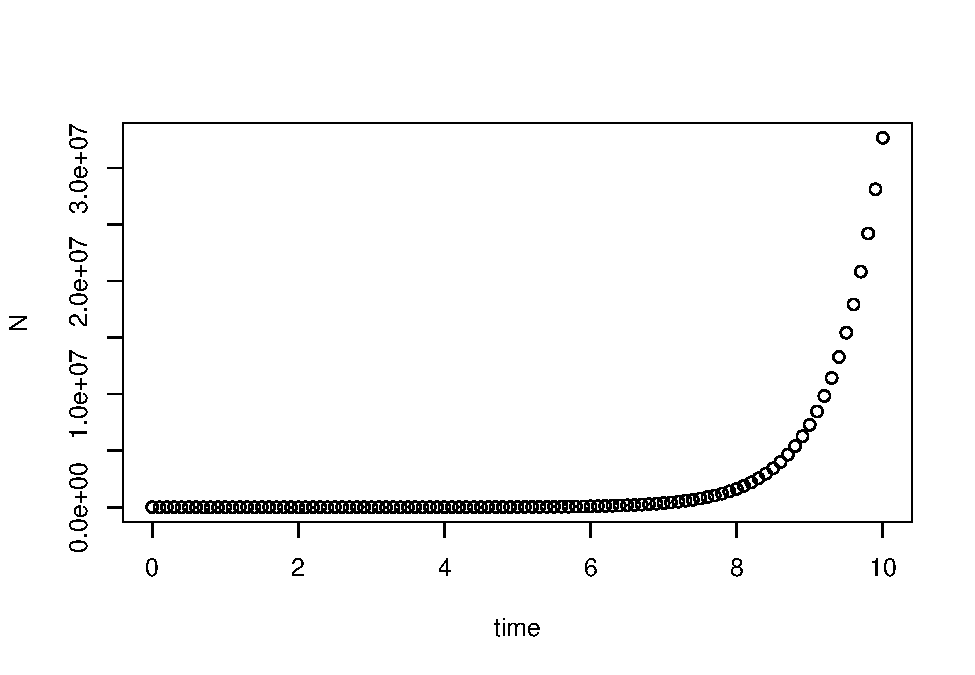
\includegraphics{bookdown-demo_files/figure-latex/unnamed-chunk-5-1.pdf}

\begin{Shaded}
\begin{Highlighting}[]
\FunctionTok{plot}\NormalTok{(N }\SpecialCharTok{\textasciitilde{}}\NormalTok{ time, }\AttributeTok{data =}\NormalTok{ pop\_size, }\AttributeTok{log =} \StringTok{"y"}\NormalTok{)}
\end{Highlighting}
\end{Shaded}

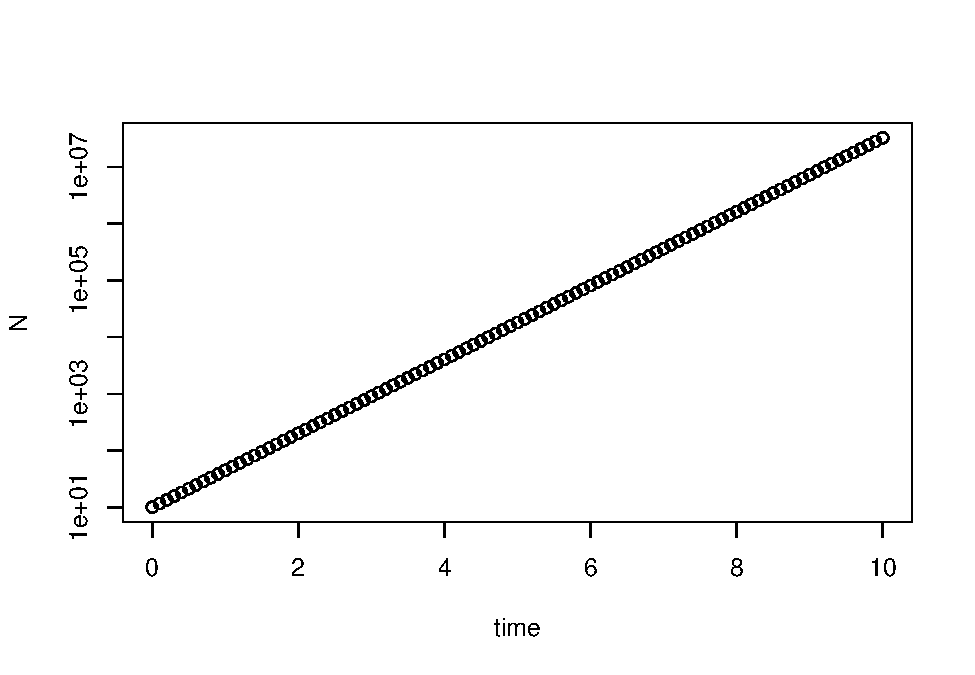
\includegraphics{bookdown-demo_files/figure-latex/unnamed-chunk-5-2.pdf}

\textbf{Part 2 - Comparing different ode solvers}
In default of \texttt{ode()}, the equations are solved by LSODA method. We can change the method by modifying the argument \texttt{method} in \texttt{ode()}.

\begin{Shaded}
\begin{Highlighting}[]
\DocumentationTok{\#\#\#\#\#\# part 2 \#\#\#\#\#\#}
\CommentTok{\# original setting}
\NormalTok{times }\OtherTok{\textless{}{-}} \FunctionTok{seq}\NormalTok{(}\DecValTok{0}\NormalTok{, }\DecValTok{10}\NormalTok{, }\AttributeTok{by =} \FloatTok{0.1}\NormalTok{)  }\CommentTok{\# time steps to integrate over}
\NormalTok{state }\OtherTok{\textless{}{-}} \FunctionTok{c}\NormalTok{(}\AttributeTok{N =} \DecValTok{10}\NormalTok{)  }\CommentTok{\# initial population size}
\NormalTok{parms }\OtherTok{\textless{}{-}} \FunctionTok{c}\NormalTok{(}\AttributeTok{r =} \FloatTok{1.5}\NormalTok{)  }\CommentTok{\# intrinsic growth rate}
\CommentTok{\# default: LSODA}
\NormalTok{pop\_size }\OtherTok{\textless{}{-}} \FunctionTok{ode}\NormalTok{(}\AttributeTok{func =}\NormalTok{ exponential\_model, }\AttributeTok{times =}\NormalTok{ times, }\AttributeTok{y =}\NormalTok{ state, }\AttributeTok{parms =}\NormalTok{ parms)}

\CommentTok{\# Euler\textquotesingle{}s method}
\NormalTok{pop\_size\_1 }\OtherTok{\textless{}{-}} \FunctionTok{ode}\NormalTok{(}\AttributeTok{func =}\NormalTok{ exponential\_model, }\AttributeTok{times =}\NormalTok{ times, }\AttributeTok{y =}\NormalTok{ state, }\AttributeTok{parms =}\NormalTok{ parms, }\AttributeTok{method =} \StringTok{"euler"}\NormalTok{)}

\CommentTok{\# compare different method}
\FunctionTok{par}\NormalTok{(}\AttributeTok{mfrow =} \FunctionTok{c}\NormalTok{(}\DecValTok{1}\NormalTok{,}\DecValTok{2}\NormalTok{))}
\FunctionTok{plot}\NormalTok{(N }\SpecialCharTok{\textasciitilde{}}\NormalTok{ time, }\AttributeTok{data =}\NormalTok{ pop\_size, }\AttributeTok{main =} \StringTok{"LSODA"}\NormalTok{)}
\FunctionTok{curve}\NormalTok{(state[}\DecValTok{1}\NormalTok{]}\SpecialCharTok{*}\FunctionTok{exp}\NormalTok{(parms[}\DecValTok{1}\NormalTok{]}\SpecialCharTok{*}\NormalTok{x), times[}\DecValTok{1}\NormalTok{], times[}\FunctionTok{length}\NormalTok{(times)], }\AttributeTok{col =} \StringTok{"red"}\NormalTok{, }\AttributeTok{add =}\NormalTok{ T) }\CommentTok{\# correct curve}
\FunctionTok{plot}\NormalTok{(N }\SpecialCharTok{\textasciitilde{}}\NormalTok{ time, }\AttributeTok{data =}\NormalTok{ pop\_size\_1, }\AttributeTok{main =} \StringTok{"Euler"}\NormalTok{)}
\FunctionTok{curve}\NormalTok{(state[}\DecValTok{1}\NormalTok{]}\SpecialCharTok{*}\FunctionTok{exp}\NormalTok{(parms[}\DecValTok{1}\NormalTok{]}\SpecialCharTok{*}\NormalTok{x), times[}\DecValTok{1}\NormalTok{], times[}\FunctionTok{length}\NormalTok{(times)], }\AttributeTok{col =} \StringTok{"red"}\NormalTok{, }\AttributeTok{add =}\NormalTok{ T) }\CommentTok{\# correct curve}
\end{Highlighting}
\end{Shaded}

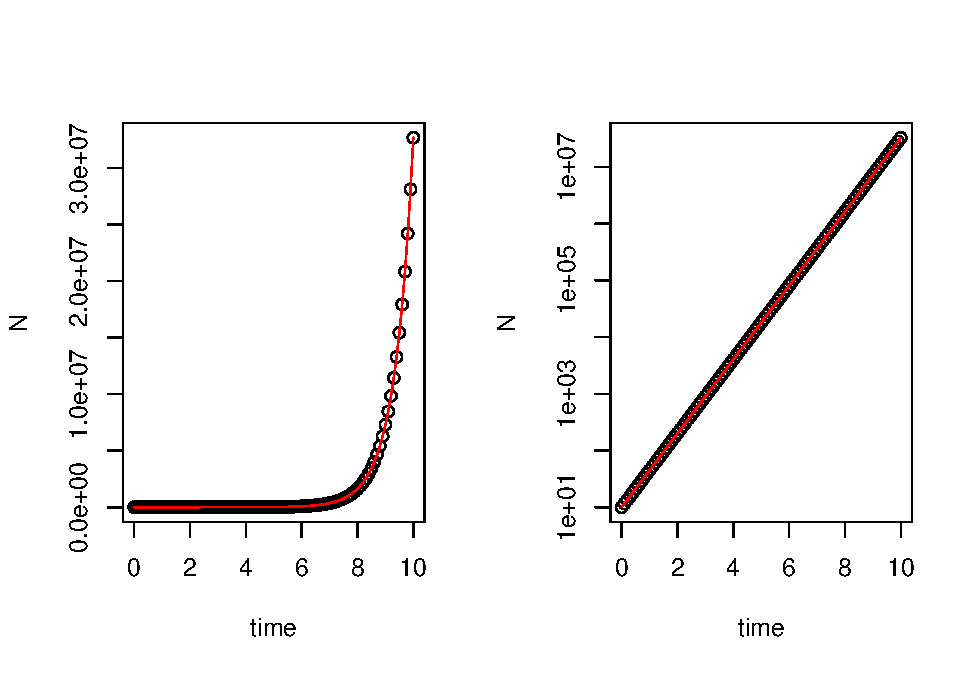
\includegraphics{bookdown-demo_files/figure-latex/unnamed-chunk-6-1.pdf}

\begin{Shaded}
\begin{Highlighting}[]
\CommentTok{\# minimize the time step}
\NormalTok{times }\OtherTok{\textless{}{-}} \FunctionTok{seq}\NormalTok{(}\DecValTok{0}\NormalTok{, }\DecValTok{10}\NormalTok{, }\AttributeTok{by =} \FloatTok{0.01}\NormalTok{)  }\CommentTok{\# time steps to integrate over}
\NormalTok{state }\OtherTok{\textless{}{-}} \FunctionTok{c}\NormalTok{(}\AttributeTok{N =} \DecValTok{10}\NormalTok{)  }\CommentTok{\# initial population size}
\NormalTok{parms }\OtherTok{\textless{}{-}} \FunctionTok{c}\NormalTok{(}\AttributeTok{r =} \FloatTok{1.5}\NormalTok{)  }\CommentTok{\# intrinsic growth rate}
\CommentTok{\# default: LSODA}
\NormalTok{pop\_size }\OtherTok{\textless{}{-}} \FunctionTok{ode}\NormalTok{(}\AttributeTok{func =}\NormalTok{ exponential\_model, }\AttributeTok{times =}\NormalTok{ times, }\AttributeTok{y =}\NormalTok{ state, }\AttributeTok{parms =}\NormalTok{ parms)}

\CommentTok{\# Euler\textquotesingle{}s method}
\NormalTok{pop\_size\_1 }\OtherTok{\textless{}{-}} \FunctionTok{ode}\NormalTok{(}\AttributeTok{func =}\NormalTok{ exponential\_model, }\AttributeTok{times =}\NormalTok{ times, }\AttributeTok{y =}\NormalTok{ state, }\AttributeTok{parms =}\NormalTok{ parms, }\AttributeTok{method =} \StringTok{"euler"}\NormalTok{)}

\CommentTok{\# compare different method}
\FunctionTok{par}\NormalTok{(}\AttributeTok{mfrow =} \FunctionTok{c}\NormalTok{(}\DecValTok{1}\NormalTok{,}\DecValTok{2}\NormalTok{))}
\FunctionTok{plot}\NormalTok{(N }\SpecialCharTok{\textasciitilde{}}\NormalTok{ time, }\AttributeTok{data =}\NormalTok{ pop\_size, }\AttributeTok{main =} \StringTok{"LSODA"}\NormalTok{)}
\FunctionTok{curve}\NormalTok{(state[}\DecValTok{1}\NormalTok{]}\SpecialCharTok{*}\FunctionTok{exp}\NormalTok{(parms[}\DecValTok{1}\NormalTok{]}\SpecialCharTok{*}\NormalTok{x), times[}\DecValTok{1}\NormalTok{], times[}\FunctionTok{length}\NormalTok{(times)], }\AttributeTok{col =} \StringTok{"red"}\NormalTok{, }\AttributeTok{add =}\NormalTok{ T) }\CommentTok{\# correct curve}
\FunctionTok{plot}\NormalTok{(N }\SpecialCharTok{\textasciitilde{}}\NormalTok{ time, }\AttributeTok{data =}\NormalTok{ pop\_size\_1, }\AttributeTok{main =} \StringTok{"Euler"}\NormalTok{)}
\FunctionTok{curve}\NormalTok{(state[}\DecValTok{1}\NormalTok{]}\SpecialCharTok{*}\FunctionTok{exp}\NormalTok{(parms[}\DecValTok{1}\NormalTok{]}\SpecialCharTok{*}\NormalTok{x), times[}\DecValTok{1}\NormalTok{], times[}\FunctionTok{length}\NormalTok{(times)], }\AttributeTok{col =} \StringTok{"red"}\NormalTok{, }\AttributeTok{add =}\NormalTok{ T) }\CommentTok{\# correct curve}
\end{Highlighting}
\end{Shaded}

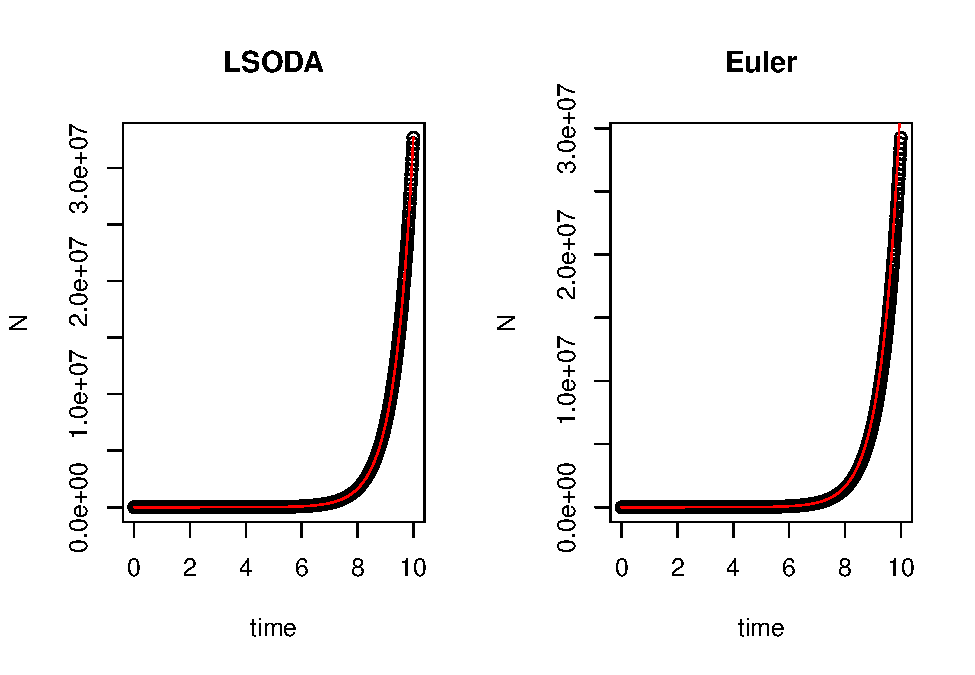
\includegraphics{bookdown-demo_files/figure-latex/unnamed-chunk-6-2.pdf}

\textbf{Part 3 - Solving exponential growth model with fluctuating growth rate}
Consider the model
\[
\frac{dN}{dt} = r(t)N \ \text{, } r(t) = \overline{r} + \sigma\sin(\omega t)
\]
where \(\overline{r}\) and \(\omega\) are constants.
The analytical solution of the ode model is
\[
N(t) = N_0\exp\{\overline{r}t - \frac{\sigma}{\omega}[\cos(\omega t) - 1]\}
\]

\begin{Shaded}
\begin{Highlighting}[]
\DocumentationTok{\#\#\#\#\#\# part 3 \#\#\#\#\#\#}
\DocumentationTok{\#\#\# Model specification}
\NormalTok{exponential\_model\_fluc }\OtherTok{\textless{}{-}} \ControlFlowTok{function}\NormalTok{(times, state, parms) \{}
  \FunctionTok{with}\NormalTok{(}\FunctionTok{as.list}\NormalTok{(}\FunctionTok{c}\NormalTok{(state, parms)), \{}
\NormalTok{    dN\_dt }\OtherTok{=}\NormalTok{ (r\_bar }\SpecialCharTok{+}\NormalTok{ sigma}\SpecialCharTok{*}\FunctionTok{sin}\NormalTok{(omega}\SpecialCharTok{*}\NormalTok{times))}\SpecialCharTok{*}\NormalTok{N  }\CommentTok{\# exponential growth equation}
    \FunctionTok{return}\NormalTok{(}\FunctionTok{list}\NormalTok{(}\FunctionTok{c}\NormalTok{(dN\_dt)))  }\CommentTok{\# return the results}
\NormalTok{  \})}
\NormalTok{\}}
\end{Highlighting}
\end{Shaded}

\begin{Shaded}
\begin{Highlighting}[]
\DocumentationTok{\#\#\# Parameters}
\NormalTok{times }\OtherTok{\textless{}{-}} \FunctionTok{seq}\NormalTok{(}\DecValTok{0}\NormalTok{, }\DecValTok{10}\NormalTok{, }\AttributeTok{by =} \FloatTok{0.1}\NormalTok{)  }\CommentTok{\# time steps to integrate over}
\NormalTok{state }\OtherTok{\textless{}{-}} \FunctionTok{c}\NormalTok{(}\AttributeTok{N =} \DecValTok{10}\NormalTok{)  }\CommentTok{\# initial population size}
\NormalTok{parms }\OtherTok{\textless{}{-}} \FunctionTok{c}\NormalTok{(}\AttributeTok{r\_bar =} \FloatTok{1.5}\NormalTok{, }\AttributeTok{sigma =} \DecValTok{5}\NormalTok{, }\AttributeTok{omega =} \DecValTok{2}\SpecialCharTok{*}\NormalTok{pi)  }\CommentTok{\# intrinsic growth rate}
\end{Highlighting}
\end{Shaded}

Plot \(r(t)\)

\begin{Shaded}
\begin{Highlighting}[]
\DocumentationTok{\#\#\# Fluctuating growth rate}
\NormalTok{r }\OtherTok{=}\NormalTok{ parms[}\DecValTok{1}\NormalTok{] }\SpecialCharTok{+}\NormalTok{ parms[}\DecValTok{2}\NormalTok{]}\SpecialCharTok{*}\FunctionTok{sin}\NormalTok{(parms[}\DecValTok{3}\NormalTok{]}\SpecialCharTok{*}\NormalTok{times)}
\FunctionTok{plot}\NormalTok{(r }\SpecialCharTok{\textasciitilde{}}\NormalTok{ times, }\AttributeTok{type =} \StringTok{"l"}\NormalTok{)}
\end{Highlighting}
\end{Shaded}

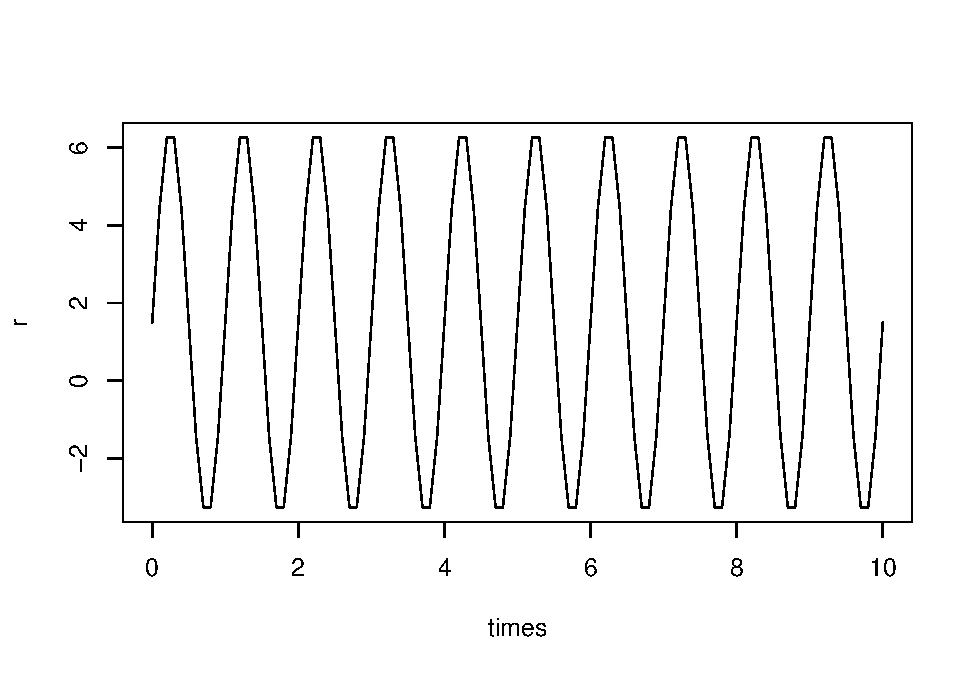
\includegraphics{bookdown-demo_files/figure-latex/unnamed-chunk-9-1.pdf}

\begin{Shaded}
\begin{Highlighting}[]
\DocumentationTok{\#\#\# Solving model}
\NormalTok{pop\_size }\OtherTok{\textless{}{-}} \FunctionTok{ode}\NormalTok{(}\AttributeTok{func =}\NormalTok{ exponential\_model\_fluc, }\AttributeTok{times =}\NormalTok{ times, }\AttributeTok{y =}\NormalTok{ state, }\AttributeTok{parms =}\NormalTok{ parms)}

\DocumentationTok{\#\#\# Plotting}
\FunctionTok{plot}\NormalTok{(N }\SpecialCharTok{\textasciitilde{}}\NormalTok{ times, }\AttributeTok{data =}\NormalTok{ pop\_size)}
\FunctionTok{curve}\NormalTok{(state[}\DecValTok{1}\NormalTok{]}\SpecialCharTok{*}\FunctionTok{exp}\NormalTok{(parms[}\DecValTok{1}\NormalTok{]}\SpecialCharTok{*}\NormalTok{x }\SpecialCharTok{{-}}\NormalTok{ parms[}\DecValTok{2}\NormalTok{]}\SpecialCharTok{/}\NormalTok{parms[}\DecValTok{3}\NormalTok{]}\SpecialCharTok{*}\NormalTok{(}\FunctionTok{cos}\NormalTok{(parms[}\DecValTok{3}\NormalTok{]}\SpecialCharTok{*}\NormalTok{x) }\SpecialCharTok{{-}} \DecValTok{1}\NormalTok{)), }\AttributeTok{add =}\NormalTok{ T, }\AttributeTok{col =} \StringTok{"red"}\NormalTok{) }\CommentTok{\# correct curve}
\end{Highlighting}
\end{Shaded}

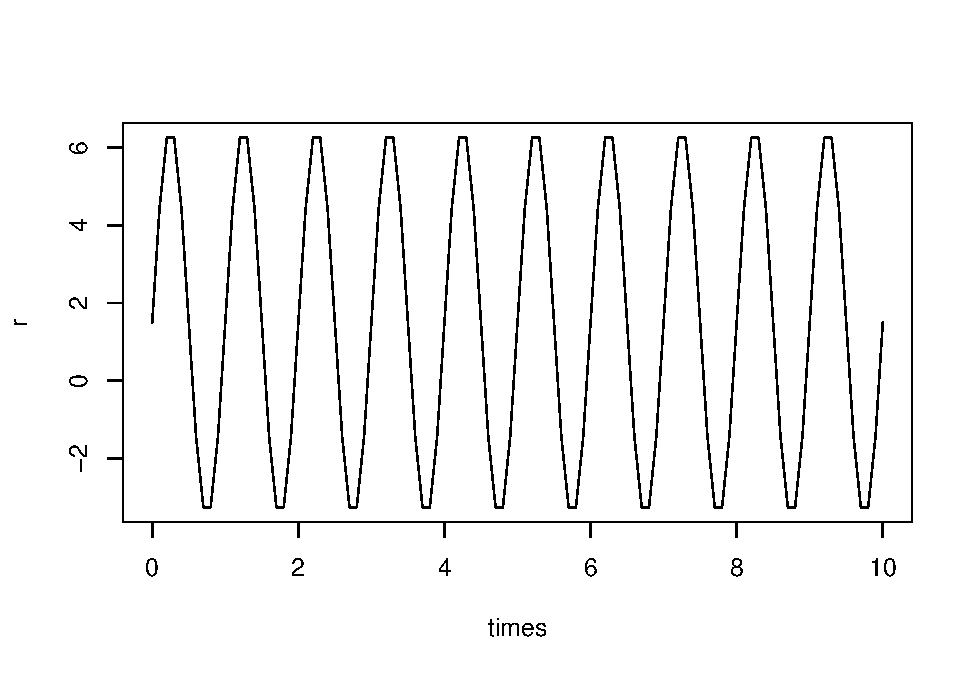
\includegraphics{bookdown-demo_files/figure-latex/unnamed-chunk-10-1.pdf}

\begin{Shaded}
\begin{Highlighting}[]
\FunctionTok{plot}\NormalTok{(N }\SpecialCharTok{\textasciitilde{}}\NormalTok{ times, }\AttributeTok{data =}\NormalTok{ pop\_size, }\AttributeTok{log =} \StringTok{"y"}\NormalTok{)}
\FunctionTok{curve}\NormalTok{(state[}\DecValTok{1}\NormalTok{]}\SpecialCharTok{*}\FunctionTok{exp}\NormalTok{(parms[}\DecValTok{1}\NormalTok{]}\SpecialCharTok{*}\NormalTok{x }\SpecialCharTok{{-}}\NormalTok{ parms[}\DecValTok{2}\NormalTok{]}\SpecialCharTok{/}\NormalTok{parms[}\DecValTok{3}\NormalTok{]}\SpecialCharTok{*}\NormalTok{(}\FunctionTok{cos}\NormalTok{(parms[}\DecValTok{3}\NormalTok{]}\SpecialCharTok{*}\NormalTok{x) }\SpecialCharTok{{-}} \DecValTok{1}\NormalTok{)), }\AttributeTok{add =}\NormalTok{ T, }\AttributeTok{col =} \StringTok{"red"}\NormalTok{) }\CommentTok{\# correct curve}
\end{Highlighting}
\end{Shaded}

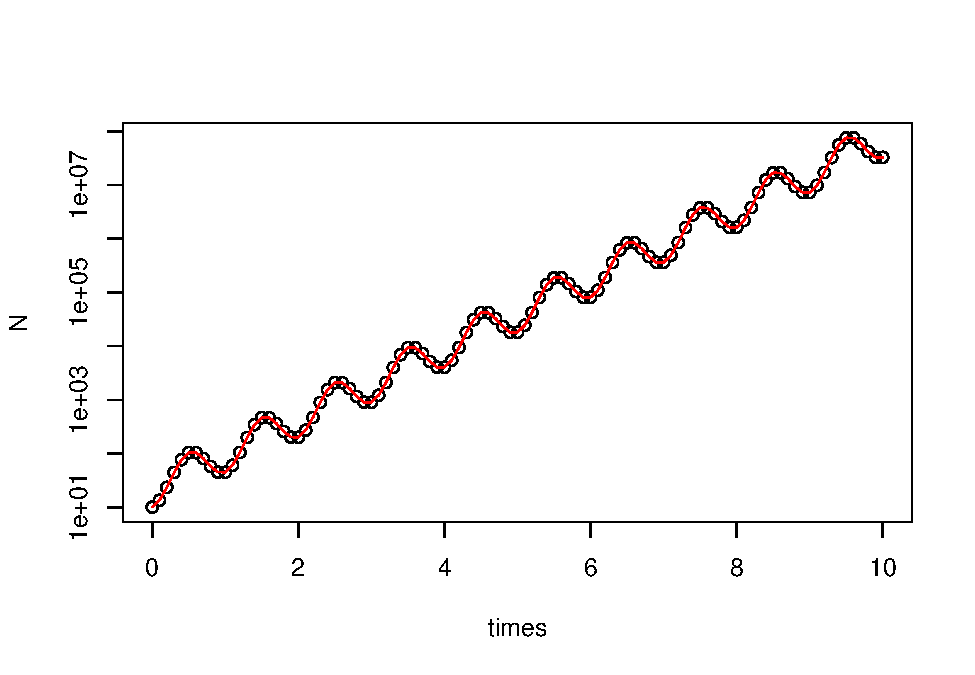
\includegraphics{bookdown-demo_files/figure-latex/unnamed-chunk-10-2.pdf}

Adjust \(\overline{r}\)

\begin{Shaded}
\begin{Highlighting}[]
\DocumentationTok{\#\#\# Parameters}
\NormalTok{times }\OtherTok{\textless{}{-}} \FunctionTok{seq}\NormalTok{(}\DecValTok{0}\NormalTok{, }\DecValTok{10}\NormalTok{, }\AttributeTok{by =} \FloatTok{0.1}\NormalTok{)  }\CommentTok{\# time steps to integrate over}
\NormalTok{state }\OtherTok{\textless{}{-}} \FunctionTok{c}\NormalTok{(}\AttributeTok{N =} \DecValTok{10}\NormalTok{)  }\CommentTok{\# initial population size}
\NormalTok{parms }\OtherTok{\textless{}{-}} \FunctionTok{c}\NormalTok{(}\AttributeTok{r\_bar =} \FloatTok{0.1}\NormalTok{, }\AttributeTok{sigma =} \DecValTok{5}\NormalTok{, }\AttributeTok{omega =} \DecValTok{2}\SpecialCharTok{*}\NormalTok{pi)  }\CommentTok{\# intrinsic growth rate}

\DocumentationTok{\#\#\# Fluctuating growth rate}
\NormalTok{r }\OtherTok{=}\NormalTok{ parms[}\DecValTok{1}\NormalTok{] }\SpecialCharTok{+}\NormalTok{ parms[}\DecValTok{2}\NormalTok{]}\SpecialCharTok{*}\FunctionTok{sin}\NormalTok{(parms[}\DecValTok{3}\NormalTok{]}\SpecialCharTok{*}\NormalTok{times)}
\FunctionTok{plot}\NormalTok{(r }\SpecialCharTok{\textasciitilde{}}\NormalTok{ times, }\AttributeTok{type =} \StringTok{"l"}\NormalTok{)}
\end{Highlighting}
\end{Shaded}

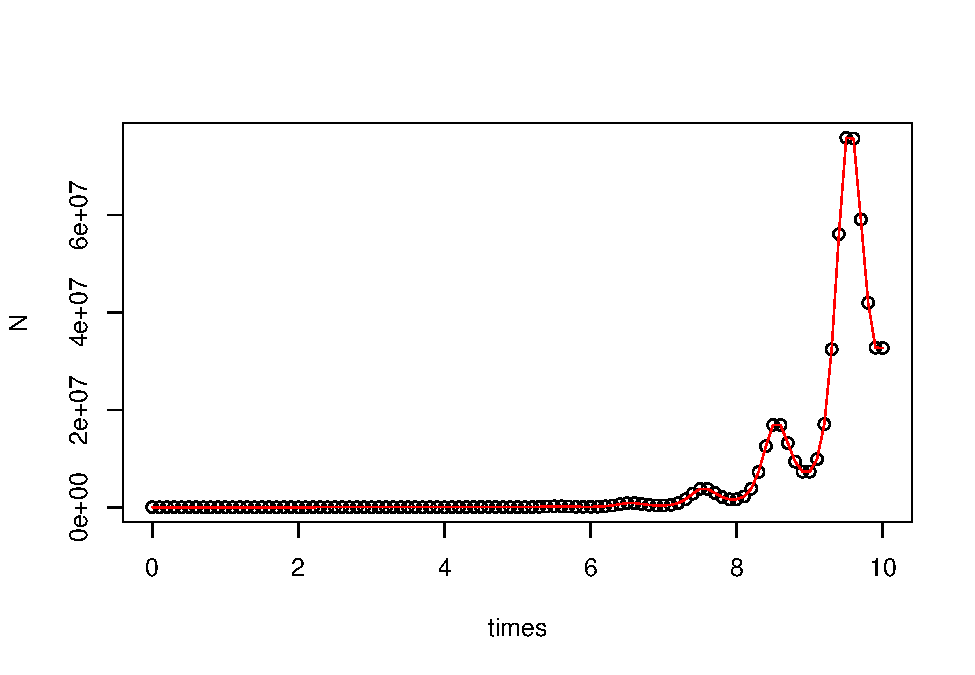
\includegraphics{bookdown-demo_files/figure-latex/unnamed-chunk-11-1.pdf}

\begin{Shaded}
\begin{Highlighting}[]
\DocumentationTok{\#\#\# Solving model}
\NormalTok{pop\_size }\OtherTok{\textless{}{-}} \FunctionTok{ode}\NormalTok{(}\AttributeTok{func =}\NormalTok{ exponential\_model\_fluc, }\AttributeTok{times =}\NormalTok{ times, }\AttributeTok{y =}\NormalTok{ state, }\AttributeTok{parms =}\NormalTok{ parms)}

\DocumentationTok{\#\#\# Plotting}
\FunctionTok{plot}\NormalTok{(N }\SpecialCharTok{\textasciitilde{}}\NormalTok{ times, }\AttributeTok{data =}\NormalTok{ pop\_size)}
\FunctionTok{curve}\NormalTok{(state[}\DecValTok{1}\NormalTok{]}\SpecialCharTok{*}\FunctionTok{exp}\NormalTok{(parms[}\DecValTok{1}\NormalTok{]}\SpecialCharTok{*}\NormalTok{x }\SpecialCharTok{{-}}\NormalTok{ parms[}\DecValTok{2}\NormalTok{]}\SpecialCharTok{/}\NormalTok{parms[}\DecValTok{3}\NormalTok{]}\SpecialCharTok{*}\NormalTok{(}\FunctionTok{cos}\NormalTok{(parms[}\DecValTok{3}\NormalTok{]}\SpecialCharTok{*}\NormalTok{x) }\SpecialCharTok{{-}} \DecValTok{1}\NormalTok{)), }\AttributeTok{add =}\NormalTok{ T, }\AttributeTok{col =} \StringTok{"red"}\NormalTok{) }\CommentTok{\# correct curve}
\end{Highlighting}
\end{Shaded}

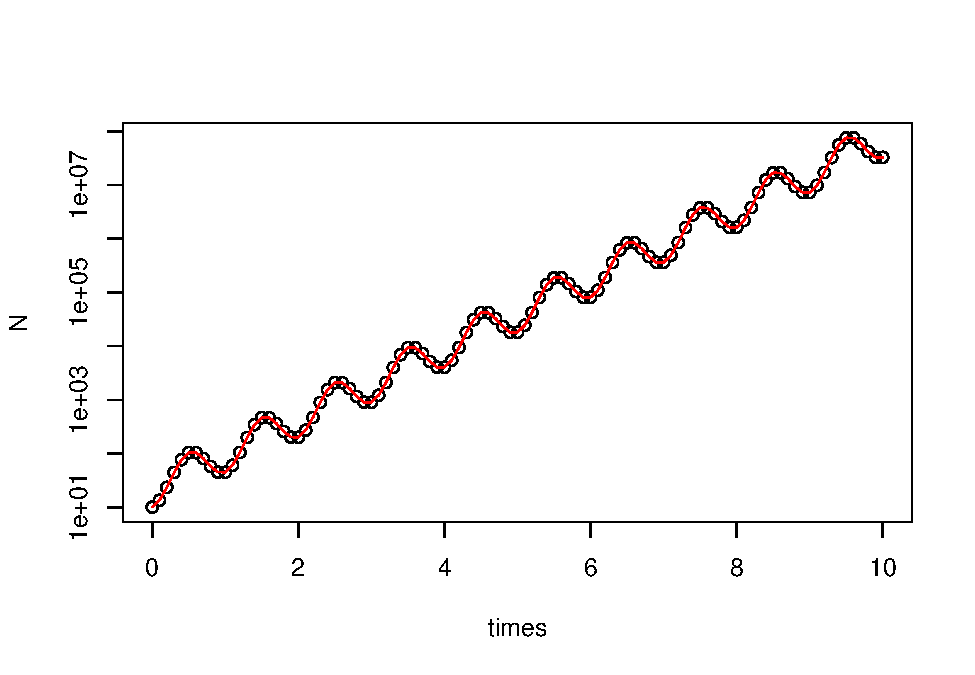
\includegraphics{bookdown-demo_files/figure-latex/unnamed-chunk-11-2.pdf}

\hypertarget{week-3---logistic-population-growth-and-stability-analysis}{%
\chapter*{Week 3 - Logistic population growth and stability analysis}\label{week-3---logistic-population-growth-and-stability-analysis}}
\addcontentsline{toc}{chapter}{Week 3 - Logistic population growth and stability analysis}

Credit to \href{https://genchanghsu.github.io/index.html}{Gen-Chang Hsu}

\hypertarget{week-4---discrete-exponential-and-logistic-models}{%
\chapter*{Week 4 - Discrete exponential and logistic models}\label{week-4---discrete-exponential-and-logistic-models}}
\addcontentsline{toc}{chapter}{Week 4 - Discrete exponential and logistic models}

\textbf{Part 1 - Model the discrete logistic population growth using for loops}
Model:
\[
N_{t+1} = N_t(1+r(1-\frac{N_t}{K}))
\]

\begin{Shaded}
\begin{Highlighting}[]
\DocumentationTok{\#\#\# (1) Define the discrete logistic growth equation}
\NormalTok{log\_fun }\OtherTok{\textless{}{-}} \ControlFlowTok{function}\NormalTok{(r, N, K)\{N }\SpecialCharTok{+}\NormalTok{ r}\SpecialCharTok{*}\NormalTok{N}\SpecialCharTok{*}\NormalTok{(}\DecValTok{1}\SpecialCharTok{{-}}\NormalTok{N}\SpecialCharTok{/}\NormalTok{K)\}}
\end{Highlighting}
\end{Shaded}

You may modify \(r\) to see the change in stability of equilibrium \(K\).

\begin{Shaded}
\begin{Highlighting}[]
\DocumentationTok{\#\#\# (2) Set the parameters}
\NormalTok{r }\OtherTok{\textless{}{-}} \FloatTok{1.8}
\NormalTok{K }\OtherTok{\textless{}{-}} \DecValTok{500}
\NormalTok{N0 }\OtherTok{\textless{}{-}} \DecValTok{10}
\NormalTok{time }\OtherTok{\textless{}{-}} \DecValTok{100}

\DocumentationTok{\#\#\# (3) Use for loop to iterate over the time sequence}
\NormalTok{pop\_size }\OtherTok{\textless{}{-}} \FunctionTok{data.frame}\NormalTok{(}\AttributeTok{times =} \DecValTok{1}\SpecialCharTok{:}\NormalTok{time)}
\NormalTok{pop\_size}\SpecialCharTok{$}\NormalTok{N[}\DecValTok{1}\NormalTok{] }\OtherTok{\textless{}{-}}\NormalTok{ N0}
\FunctionTok{head}\NormalTok{(pop\_size)}
\end{Highlighting}
\end{Shaded}

\begin{verbatim}
##   times  N
## 1     1 10
## 2     2 10
## 3     3 10
## 4     4 10
## 5     5 10
## 6     6 10
\end{verbatim}

\begin{Shaded}
\begin{Highlighting}[]
\ControlFlowTok{for}\NormalTok{(i }\ControlFlowTok{in} \DecValTok{2}\SpecialCharTok{:}\NormalTok{time)\{}
\NormalTok{  pop\_size}\SpecialCharTok{$}\NormalTok{N[i] }\OtherTok{\textless{}{-}} \FunctionTok{log\_fun}\NormalTok{(}\AttributeTok{r =}\NormalTok{ r, }\AttributeTok{N =}\NormalTok{ pop\_size}\SpecialCharTok{$}\NormalTok{N[i }\SpecialCharTok{{-}} \DecValTok{1}\NormalTok{], }\AttributeTok{K =}\NormalTok{ K)}
\NormalTok{\}}

\FunctionTok{head}\NormalTok{(pop\_size)}
\end{Highlighting}
\end{Shaded}

\begin{verbatim}
##   times         N
## 1     1  10.00000
## 2     2  27.64000
## 3     3  74.64171
## 4     4 188.93980
## 5     5 400.51775
## 6     6 543.95762
\end{verbatim}

\begin{Shaded}
\begin{Highlighting}[]
\DocumentationTok{\#\#\# (4) Population trajectory}
\FunctionTok{plot}\NormalTok{(N }\SpecialCharTok{\textasciitilde{}}\NormalTok{ times, }\AttributeTok{data =}\NormalTok{ pop\_size, }\AttributeTok{type =} \StringTok{"l"}\NormalTok{)}
\FunctionTok{abline}\NormalTok{(}\AttributeTok{h =}\NormalTok{ K, }\AttributeTok{col =} \StringTok{"red"}\NormalTok{)}
\FunctionTok{points}\NormalTok{(N }\SpecialCharTok{\textasciitilde{}}\NormalTok{ times, }\AttributeTok{data =}\NormalTok{ pop\_size)}
\end{Highlighting}
\end{Shaded}

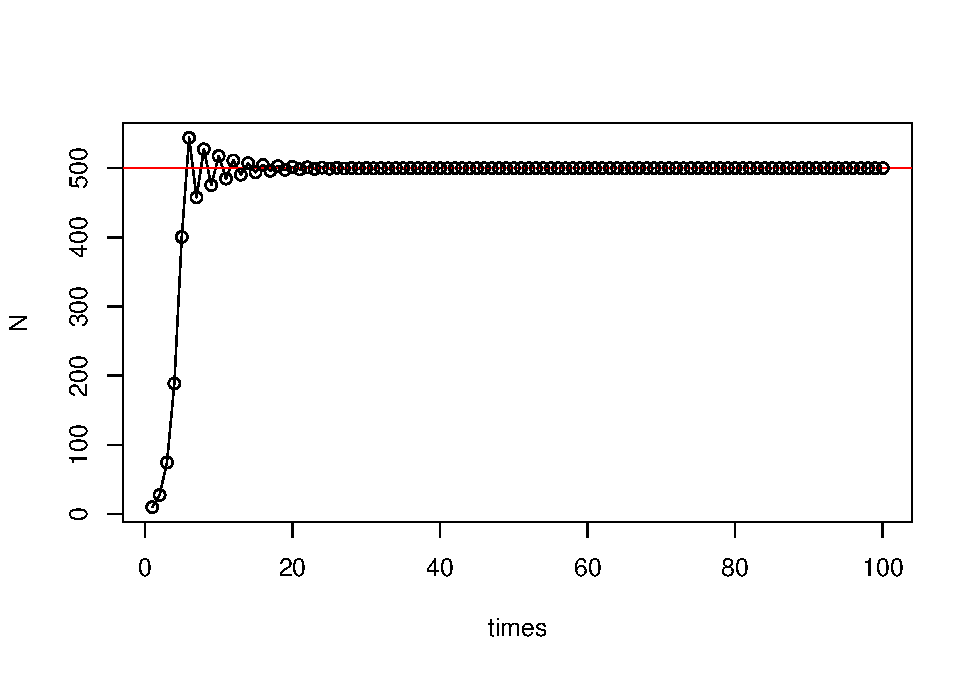
\includegraphics{bookdown-demo_files/figure-latex/unnamed-chunk-14-1.pdf}

Here is a shiny app for the discrete logistic growth model.

Credit to \href{https://genchanghsu.github.io/index.html}{Gen-Chang Hsu}

\textbf{Part 2 - Bifurcation}

\begin{Shaded}
\begin{Highlighting}[]
\DocumentationTok{\#\#\#\#\#\# Part 2: Bifurcation curve}
\DocumentationTok{\#\#\# (1) data setting}
\CommentTok{\# intrinsic growth rate sequence}
\NormalTok{r\_seq }\OtherTok{\textless{}{-}} \FunctionTok{seq}\NormalTok{(}\AttributeTok{from =} \FloatTok{1.8}\NormalTok{, }\AttributeTok{to =} \DecValTok{3}\NormalTok{, }\AttributeTok{by =} \FloatTok{0.01}\NormalTok{)}
\CommentTok{\# number of sampling}
\NormalTok{N\_rep }\OtherTok{\textless{}{-}} \DecValTok{200}

\CommentTok{\# data }
\NormalTok{dat\_plot }\OtherTok{\textless{}{-}} \FunctionTok{data.frame}\NormalTok{(}\AttributeTok{r =} \FunctionTok{rep}\NormalTok{(r\_seq, }\AttributeTok{each =}\NormalTok{ N\_rep), }\AttributeTok{N =} \DecValTok{0}\NormalTok{)}
\FunctionTok{head}\NormalTok{(dat\_plot)}
\end{Highlighting}
\end{Shaded}

\begin{verbatim}
##     r N
## 1 1.8 0
## 2 1.8 0
## 3 1.8 0
## 4 1.8 0
## 5 1.8 0
## 6 1.8 0
\end{verbatim}

\begin{Shaded}
\begin{Highlighting}[]
\DocumentationTok{\#\#\# (2) Run the discrete logistic model}
\ControlFlowTok{for}\NormalTok{ (lo }\ControlFlowTok{in} \DecValTok{1}\SpecialCharTok{:}\FunctionTok{length}\NormalTok{(r\_seq))\{}
\NormalTok{  log\_fun }\OtherTok{\textless{}{-}} \ControlFlowTok{function}\NormalTok{(r, N, K)\{N }\SpecialCharTok{+}\NormalTok{ r}\SpecialCharTok{*}\NormalTok{N}\SpecialCharTok{*}\NormalTok{(}\DecValTok{1}\SpecialCharTok{{-}}\NormalTok{N}\SpecialCharTok{/}\NormalTok{K)\}}

\NormalTok{  r }\OtherTok{\textless{}{-}}\NormalTok{ r\_seq[lo]}
\NormalTok{  K }\OtherTok{\textless{}{-}} \DecValTok{500}
\NormalTok{  N0 }\OtherTok{\textless{}{-}} \DecValTok{10}
\NormalTok{  time }\OtherTok{\textless{}{-}} \DecValTok{1000}

\NormalTok{  pop\_size }\OtherTok{\textless{}{-}} \FunctionTok{data.frame}\NormalTok{(}\AttributeTok{times =} \DecValTok{1}\SpecialCharTok{:}\NormalTok{time)}
\NormalTok{  pop\_size}\SpecialCharTok{$}\NormalTok{N[}\DecValTok{1}\NormalTok{] }\OtherTok{\textless{}{-}}\NormalTok{ N0}

  \ControlFlowTok{for}\NormalTok{(i }\ControlFlowTok{in} \DecValTok{2}\SpecialCharTok{:}\NormalTok{time)\{}
\NormalTok{    pop\_size}\SpecialCharTok{$}\NormalTok{N[i] }\OtherTok{\textless{}{-}} \FunctionTok{log\_fun}\NormalTok{(}\AttributeTok{r =}\NormalTok{ r, }\AttributeTok{N =}\NormalTok{ pop\_size}\SpecialCharTok{$}\NormalTok{N[i }\SpecialCharTok{{-}} \DecValTok{1}\NormalTok{], }\AttributeTok{K =}\NormalTok{ K)}
\NormalTok{  \}}

  \CommentTok{\# save the data}
\NormalTok{  dat\_plot}\SpecialCharTok{$}\NormalTok{N[(}\DecValTok{1} \SpecialCharTok{+}\NormalTok{ (lo }\SpecialCharTok{{-}} \DecValTok{1}\NormalTok{)}\SpecialCharTok{*}\NormalTok{N\_rep)}\SpecialCharTok{:}\NormalTok{(lo}\SpecialCharTok{*}\NormalTok{N\_rep)] }\OtherTok{\textless{}{-}}\NormalTok{ pop\_size}\SpecialCharTok{$}\NormalTok{N[(}\FunctionTok{nrow}\NormalTok{(pop\_size) }\SpecialCharTok{{-}}\NormalTok{ N\_rep }\SpecialCharTok{+} \DecValTok{1}\NormalTok{)}\SpecialCharTok{:}\FunctionTok{nrow}\NormalTok{(pop\_size)]}
\NormalTok{\}}

\FunctionTok{plot}\NormalTok{(N }\SpecialCharTok{\textasciitilde{}}\NormalTok{ r, }\AttributeTok{data =}\NormalTok{ dat\_plot, }\AttributeTok{cex =} \FloatTok{0.7}\NormalTok{, }\AttributeTok{pch =} \DecValTok{20}\NormalTok{)}
\end{Highlighting}
\end{Shaded}

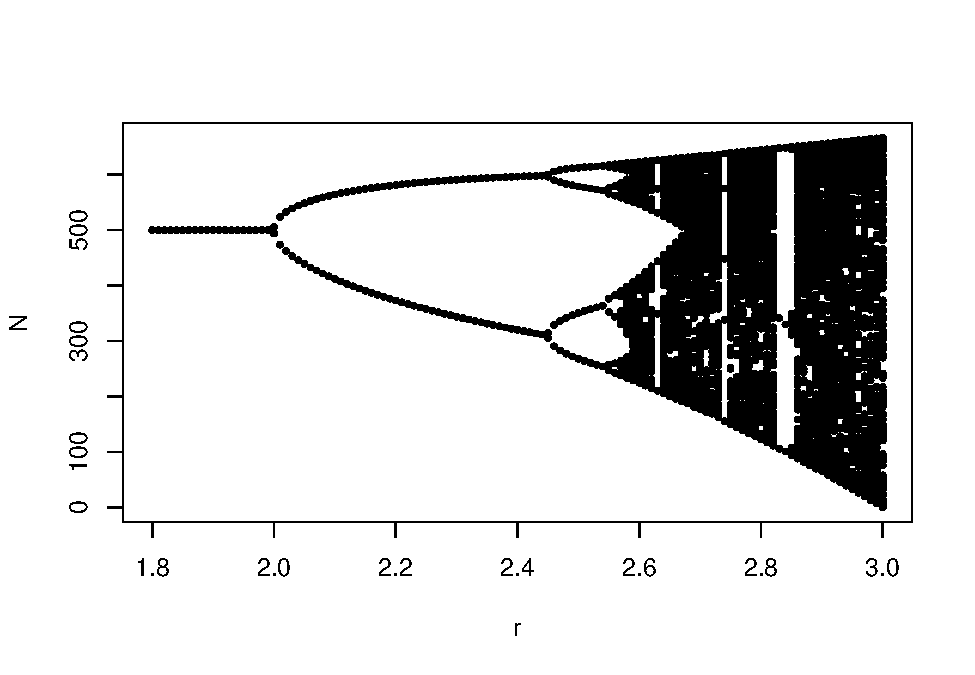
\includegraphics{bookdown-demo_files/figure-latex/unnamed-chunk-16-1.pdf}

\hypertarget{week-5---age-structure-population-model}{%
\chapter*{Week 5 - Age-structure population model}\label{week-5---age-structure-population-model}}
\addcontentsline{toc}{chapter}{Week 5 - Age-structure population model}

In this lab section, we will analyze a Leslie matrix using for loops and matrix algebra, compare the results with those obtained via eigen-analysis, and visualize the population dynamics and age distribution.

\textbf{Part 1 - Visualizing stable age distribution}

For any diagonalizable n-by-n matrix \(M\) with only one dominant eigenvalue, and for any n-by-1 vector \(v\), \(M^tv\) will shift to the same direction with the eigenvector of \(M\) corresponding to the dominant eigenvalue when \(t\) is large. Here, we visualize this fact numerically.

\begin{Shaded}
\begin{Highlighting}[]
\FunctionTok{library}\NormalTok{(ggplot2)}
\FunctionTok{set.seed}\NormalTok{(}\DecValTok{1234}\NormalTok{)}
\NormalTok{MAT }\OtherTok{\textless{}{-}} \FunctionTok{matrix}\NormalTok{(}\FunctionTok{rnorm}\NormalTok{(}\DecValTok{25}\NormalTok{), }\AttributeTok{ncol =} \DecValTok{5}\NormalTok{, }\AttributeTok{nrow =} \DecValTok{5}\NormalTok{)}
\FunctionTok{abs}\NormalTok{(}\FunctionTok{eigen}\NormalTok{(MAT)}\SpecialCharTok{$}\NormalTok{values) }\CommentTok{\# check only one dominant eigenvalue}
\end{Highlighting}
\end{Shaded}

\begin{verbatim}
## [1] 2.2734833 1.6266143 0.6187862 0.6187862 0.3970850
\end{verbatim}

\begin{Shaded}
\begin{Highlighting}[]
\NormalTok{eig\_vec1 }\OtherTok{\textless{}{-}} \FunctionTok{as.numeric}\NormalTok{(}\FunctionTok{eigen}\NormalTok{(MAT)}\SpecialCharTok{$}\NormalTok{vector[, }\DecValTok{1}\NormalTok{])}
\NormalTok{v }\OtherTok{\textless{}{-}} \FunctionTok{rnorm}\NormalTok{(}\DecValTok{5}\NormalTok{)}
\NormalTok{time }\OtherTok{\textless{}{-}} \DecValTok{15}

\NormalTok{dat\_v }\OtherTok{\textless{}{-}} \FunctionTok{data.frame}\NormalTok{(}\FunctionTok{matrix}\NormalTok{(}\AttributeTok{ncol =} \DecValTok{5}\NormalTok{, }\AttributeTok{nrow =}\NormalTok{ time))}
\NormalTok{dat\_v[}\DecValTok{1}\NormalTok{, ] }\OtherTok{\textless{}{-}}\NormalTok{ v}
\ControlFlowTok{for}\NormalTok{(i }\ControlFlowTok{in} \DecValTok{2}\SpecialCharTok{:}\NormalTok{time)\{}
\NormalTok{  dat\_v[i, ] }\OtherTok{\textless{}{-}}\NormalTok{ MAT }\SpecialCharTok{\%*\%} \FunctionTok{t}\NormalTok{(dat\_v[i}\DecValTok{{-}1}\NormalTok{, ])}
\NormalTok{\}}

\CommentTok{\# Remake data for gganimate}
\NormalTok{dat }\OtherTok{\textless{}{-}} \FunctionTok{data.frame}\NormalTok{(}\AttributeTok{X1 =} \DecValTok{0}\NormalTok{, }\AttributeTok{X2 =} \DecValTok{0}\NormalTok{, }\AttributeTok{Time =} \DecValTok{1}\NormalTok{)}
\ControlFlowTok{for}\NormalTok{(i }\ControlFlowTok{in} \DecValTok{1}\SpecialCharTok{:}\NormalTok{time)\{}
\NormalTok{  dat }\OtherTok{\textless{}{-}} \FunctionTok{rbind}\NormalTok{(dat, }\FunctionTok{data.frame}\NormalTok{(dat\_v[i,}\DecValTok{1}\SpecialCharTok{:}\DecValTok{2}\NormalTok{] }\SpecialCharTok{/} \FunctionTok{sqrt}\NormalTok{(}\FunctionTok{sum}\NormalTok{(dat\_v[i,}\DecValTok{1}\SpecialCharTok{:}\DecValTok{2}\NormalTok{]}\SpecialCharTok{\^{}}\DecValTok{2}\NormalTok{)) }\SpecialCharTok{*}\NormalTok{ i, }\AttributeTok{Time =}\NormalTok{ i))}
\NormalTok{  dat }\OtherTok{\textless{}{-}} \FunctionTok{rbind}\NormalTok{(dat, }\FunctionTok{c}\NormalTok{(}\DecValTok{0}\NormalTok{,}\DecValTok{0}\NormalTok{, i}\SpecialCharTok{+}\DecValTok{1}\NormalTok{))}
\NormalTok{\}}
\NormalTok{dat }\OtherTok{\textless{}{-}}\NormalTok{ dat[}\SpecialCharTok{{-}}\FunctionTok{nrow}\NormalTok{(dat), ]}


\FunctionTok{ggplot}\NormalTok{(dat, }\FunctionTok{aes}\NormalTok{(X1, X2, }\AttributeTok{color =}\NormalTok{ Time)) }\SpecialCharTok{+}
  \FunctionTok{geom\_path}\NormalTok{(}\AttributeTok{arrow =} \FunctionTok{arrow}\NormalTok{(}\AttributeTok{length =} \FunctionTok{unit}\NormalTok{(}\FloatTok{0.55}\NormalTok{, }\StringTok{"cm"}\NormalTok{))) }\SpecialCharTok{+} 
  \FunctionTok{geom\_abline}\NormalTok{(}\AttributeTok{intercept =} \DecValTok{0}\NormalTok{, }
              \AttributeTok{slope =}\NormalTok{ eig\_vec1[}\DecValTok{2}\NormalTok{]}\SpecialCharTok{/}\NormalTok{eig\_vec1[}\DecValTok{1}\NormalTok{], }
              \AttributeTok{color =} \StringTok{"red"}\NormalTok{, }
              \AttributeTok{linetype =} \StringTok{"dashed"}\NormalTok{) }\CommentTok{\# red dashed eigenvector}
\end{Highlighting}
\end{Shaded}

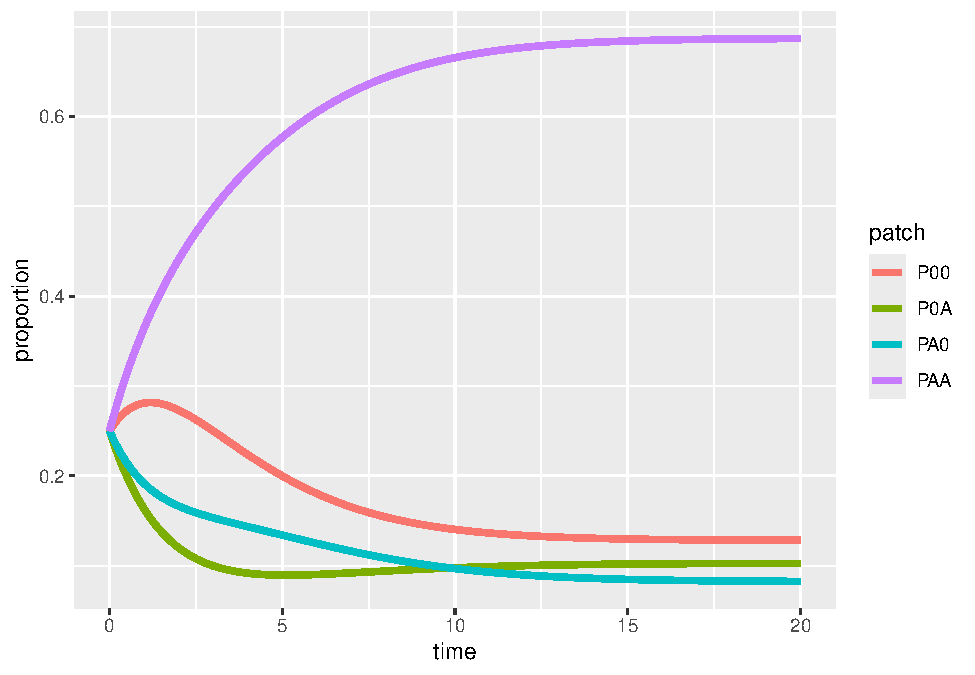
\includegraphics{bookdown-demo_files/figure-latex/unnamed-chunk-17-1.pdf}

\textbf{Part 2 - Analyzing Leslie matrix}

Consider an age-strutured population model
\[
n_{t} = L^tn_0
\]
where \(L\) is a Leslie matrix and \(n_t = (n_{1,t}, n_{2,t}, n_{3,t})\) is the population sizes with three different ages in time \(t\).

\begin{Shaded}
\begin{Highlighting}[]
\DocumentationTok{\#\#\# Leslie matrix and initial age classes}
\NormalTok{leslie }\OtherTok{\textless{}{-}} \FunctionTok{matrix}\NormalTok{(}\AttributeTok{data =} \FunctionTok{c}\NormalTok{(}\DecValTok{0}\NormalTok{, }\DecValTok{1}\NormalTok{, }\DecValTok{5}\NormalTok{,}
                          \FloatTok{0.5}\NormalTok{, }\DecValTok{0}\NormalTok{, }\DecValTok{0}\NormalTok{,}
                          \DecValTok{0}\NormalTok{, }\FloatTok{0.3}\NormalTok{, }\DecValTok{0}\NormalTok{),}
                      \AttributeTok{nrow =} \DecValTok{3}\NormalTok{,}
                      \AttributeTok{ncol =} \DecValTok{3}\NormalTok{,}
                      \AttributeTok{byrow =}\NormalTok{ T)}

\NormalTok{N0 }\OtherTok{\textless{}{-}} \FunctionTok{c}\NormalTok{(}\DecValTok{10}\NormalTok{, }\DecValTok{0}\NormalTok{, }\DecValTok{0}\NormalTok{)}

\DocumentationTok{\#\#\# for loop and matrix algebra}
\NormalTok{time }\OtherTok{\textless{}{-}} \DecValTok{50}
\NormalTok{pop\_size }\OtherTok{\textless{}{-}} \FunctionTok{data.frame}\NormalTok{(}\AttributeTok{Age1 =} \DecValTok{0}\NormalTok{,}
                       \AttributeTok{Age2 =} \DecValTok{0}\NormalTok{,}
                       \AttributeTok{Age3 =} \DecValTok{0}\NormalTok{)}
\NormalTok{pop\_size[}\DecValTok{1}\NormalTok{, ] }\OtherTok{\textless{}{-}}\NormalTok{ N0}

\ControlFlowTok{for}\NormalTok{ (i }\ControlFlowTok{in} \DecValTok{2}\SpecialCharTok{:}\NormalTok{time) \{}
  \CommentTok{\# Matrix multiplication}
\NormalTok{  pop\_size[i, ] }\OtherTok{\textless{}{-}}\NormalTok{ leslie }\SpecialCharTok{\%*\%} \FunctionTok{t}\NormalTok{(pop\_size[i}\DecValTok{{-}1}\NormalTok{, ])}
\NormalTok{\}}

\CommentTok{\# Total abundance}
\NormalTok{pop\_size}\SpecialCharTok{$}\NormalTok{N }\OtherTok{\textless{}{-}} \FunctionTok{rowSums}\NormalTok{(pop\_size)}

\FunctionTok{head}\NormalTok{(pop\_size)}
\end{Highlighting}
\end{Shaded}

\begin{verbatim}
##   Age1 Age2  Age3      N
## 1 10.0 0.00 0.000 10.000
## 2  0.0 5.00 0.000  5.000
## 3  5.0 0.00 1.500  6.500
## 4  7.5 2.50 0.000 10.000
## 5  2.5 3.75 0.750  7.000
## 6  7.5 1.25 1.125  9.875
\end{verbatim}

\begin{Shaded}
\begin{Highlighting}[]
\FunctionTok{plot}\NormalTok{(}\FunctionTok{c}\NormalTok{(}\DecValTok{1}\NormalTok{,time), }\FunctionTok{c}\NormalTok{(}\DecValTok{0}\NormalTok{,}\DecValTok{265}\NormalTok{), }\AttributeTok{type =} \StringTok{"n"}\NormalTok{, }\AttributeTok{xlab =} \StringTok{"time"}\NormalTok{, }\AttributeTok{ylab =} \StringTok{"pop\_size"}\NormalTok{)}
\FunctionTok{lines}\NormalTok{(}\DecValTok{1}\SpecialCharTok{:}\NormalTok{time , pop\_size}\SpecialCharTok{$}\NormalTok{Age1, }\AttributeTok{col =} \StringTok{"red"}\NormalTok{)}
\FunctionTok{lines}\NormalTok{(}\DecValTok{1}\SpecialCharTok{:}\NormalTok{time , pop\_size}\SpecialCharTok{$}\NormalTok{Age2, }\AttributeTok{col =} \StringTok{"blue"}\NormalTok{)}
\FunctionTok{lines}\NormalTok{(}\DecValTok{1}\SpecialCharTok{:}\NormalTok{time , pop\_size}\SpecialCharTok{$}\NormalTok{Age3, }\AttributeTok{col =} \StringTok{"green"}\NormalTok{)}
\FunctionTok{legend}\NormalTok{(}\StringTok{"topleft"}\NormalTok{,}
       \AttributeTok{legend =} \FunctionTok{c}\NormalTok{(}\StringTok{"Age1"}\NormalTok{, }\StringTok{"Age2"}\NormalTok{, }\StringTok{"Age3"}\NormalTok{),}
       \AttributeTok{col =} \FunctionTok{c}\NormalTok{(}\StringTok{"red"}\NormalTok{, }\StringTok{"blue"}\NormalTok{, }\StringTok{"green"}\NormalTok{),}
       \AttributeTok{lty =} \DecValTok{1}\NormalTok{)}
\end{Highlighting}
\end{Shaded}

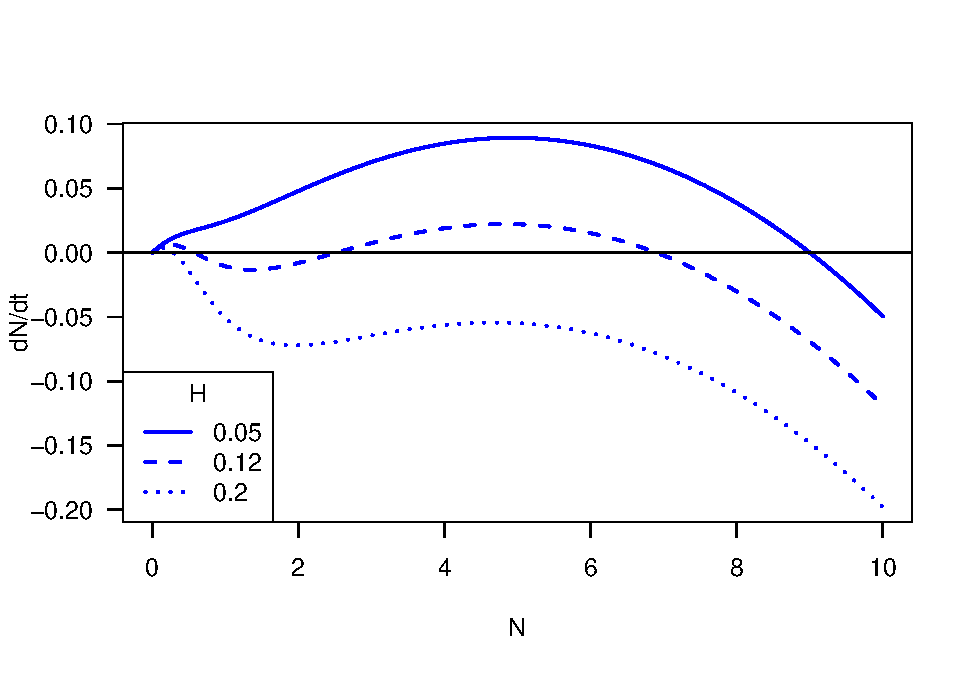
\includegraphics{bookdown-demo_files/figure-latex/unnamed-chunk-18-1.pdf}

By the derivation in the class, the asymptotic population sizes can be approximated by
\[
n_t \approx c\cdot \lambda_1^t\cdot u_1
\]
where \(c\) is a constant, \(\lambda_1\) is the dominant eigenvalue and \(u_1\) is the corresponding eigenvector. Hence, with the long-term dynamics, the population grows at a rate \(\lambda_1\) and with the age distribution \(u_1\). Here, we check this fact numerically.

\begin{Shaded}
\begin{Highlighting}[]
\DocumentationTok{\#\#\# Asymptotic growth rate and stable age distribution}

\NormalTok{asymptotic\_growth }\OtherTok{\textless{}{-}}\NormalTok{ pop\_size}\SpecialCharTok{$}\NormalTok{N[time]}\SpecialCharTok{/}\NormalTok{pop\_size}\SpecialCharTok{$}\NormalTok{N[time}\DecValTok{{-}1}\NormalTok{]}
\NormalTok{asymptotic\_growth}
\end{Highlighting}
\end{Shaded}

\begin{verbatim}
## [1] 1.089992
\end{verbatim}

\begin{Shaded}
\begin{Highlighting}[]
\NormalTok{age\_distribution }\OtherTok{\textless{}{-}}\NormalTok{ pop\_size[time, }\DecValTok{1}\SpecialCharTok{:}\DecValTok{3}\NormalTok{]}\SpecialCharTok{/}\FunctionTok{sum}\NormalTok{(pop\_size[time, }\DecValTok{1}\SpecialCharTok{:}\DecValTok{3}\NormalTok{])}
\NormalTok{age\_distribution}
\end{Highlighting}
\end{Shaded}

\begin{verbatim}
##         Age1      Age2       Age3
## 50 0.6309262 0.2894167 0.07965713
\end{verbatim}

\begin{Shaded}
\begin{Highlighting}[]
\DocumentationTok{\#\#\# Eigen{-}analysis of the Leslie matrix}
\NormalTok{EIGEN }\OtherTok{\textless{}{-}} \FunctionTok{eigen}\NormalTok{(leslie)}
\NormalTok{EIGEN}
\end{Highlighting}
\end{Shaded}

\begin{verbatim}
## eigen() decomposition
## $values
## [1]  1.0899905+0.0000000i -0.5449953+0.6253475i -0.5449953-0.6253475i
## 
## $vectors
##              [,1]                  [,2]                  [,3]
## [1,] 0.9030054+0i  0.8418972+0.0000000i  0.8418972+0.0000000i
## [2,] 0.4142263+0i -0.3334136-0.3825709i -0.3334136+0.3825709i
## [3,] 0.1140082+0i -0.0250833+0.1818099i -0.0250833-0.1818099i
\end{verbatim}

\begin{Shaded}
\begin{Highlighting}[]
\FunctionTok{abs}\NormalTok{(EIGEN}\SpecialCharTok{$}\NormalTok{values[}\DecValTok{1}\NormalTok{]) }\CommentTok{\# dominant eigenvalue}
\end{Highlighting}
\end{Shaded}

\begin{verbatim}
## [1] 1.089991
\end{verbatim}

\begin{Shaded}
\begin{Highlighting}[]
\FunctionTok{as.numeric}\NormalTok{(EIGEN}\SpecialCharTok{$}\NormalTok{vectors[, }\DecValTok{1}\NormalTok{] }\SpecialCharTok{/} \FunctionTok{sum}\NormalTok{(EIGEN}\SpecialCharTok{$}\NormalTok{vectors[, }\DecValTok{1}\NormalTok{])) }\CommentTok{\# corresponding eigenvector}
\end{Highlighting}
\end{Shaded}

\begin{verbatim}
## [1] 0.63092527 0.28941777 0.07965696
\end{verbatim}

The asymptotic growth rate and stable age distribution obtained from for loops and eigen-analysis are similar.

\textbf{Part 3 - In-class exercise: Analyzing population matrix of common teasel}

\href{https://en.wikipedia.org/wiki/Dipsacus_fullonum}{Common teasel (\emph{Dipsacus sylvestris})} is a herbaceous plant commonly found in abandoned fields and meadows in North America. It has a complex life cycle consisting of various stages. The seeds may lie dormant for one or two years. Seeds that germinate form small rosettes, which will gradually transit into medium and eventually large rosettes. These rosettes (all three sizes) may remain in the same stage for years before entering the next stage. After undergoing vernalization, large (and a few medium) rosettes will form stalks and flower in the upcoming summer, set seeds once, and die. Occasionally, the flowering plants will produce seeds that directly germinate into small/medium/large rosettes without entering dormancy.

Here is a transition diagram for the teasel. Please convert this diagram into a stage-based transition matrix (Lefkovitch matrix) and derive the asymptotic growth rate \(\lambda\) in R.

\textbf{Part 4 - COM(P)ADRE: A global database of population matrices}

\href{https://compadre-db.org/ExploreDatabase}{COM(P)ADRE} is an online repository containing matrix population models on hundreds of plants, animals, algae, fungi, bacteria, and viruses around the world, as well as their associated metadata. Take a look at the website: You will be exploring the population dynamics of a species (of your choice) in your assignment!

\hypertarget{week-6---metapopulations-and-patch-occupancy-models}{%
\chapter*{Week 6 - Metapopulations and patch occupancy models}\label{week-6---metapopulations-and-patch-occupancy-models}}
\addcontentsline{toc}{chapter}{Week 6 - Metapopulations and patch occupancy models}

Plants can condition nearby soil microbial communities, which will in turn influence the performance of subsequent colonizing plants. The soil beneath plant communities are therefore a mosaic with different cultivation histories. Po-Ju wants to understand how plant demographic rates (i.e., colonization and mortality rate) and microbial dynamics (i.e., the conditioning and decay rate of microbial communities) affect the percentage of different soil types in natural forests. As a starting point, Po-Ju builds a one-species patch occupancy model to track the dynamics of different types of plant-soil combination.

In this model, he characterizes sites by their plant-soil microbe state, using the notation \(P_{ij}\) to indicate sites that are now occupied by plant species \(i\) but have soil microbes state \(j\). Here, as a single species model, \(i\) can be 0 or \(A\), representing uncolonized sites or sites colonized by plant \(A\), respectively. Similarly, \(j\) can be 0 or \(A\), indicating sites without recent plant conditioning history or sites conditioned by plant \(A\), respectively. In summary:

\begin{enumerate}
\def\labelenumi{\arabic{enumi}.}
\tightlist
\item
  \(P_{00}\) represents uncolonized and unconditioned sites
\item
  \(P_{A0}\) represents cites colonized by plant \(A\) but the soil is yet to be conditioned
\item
  \(P_{AA}\) represents plant \(A\) colonizing a site with plant-\(A\)-specific microbial community
\item
  \(P_{0A}\) represents sites that are currently unoccupied but have soil microbes that were associated with plant \(A\)
\end{enumerate}

At the landscape scale, \(P_{ij}\) represents the proportion of sites belonging to a particular plant-soil microbe state, and its dynamics, \(\frac {dP_{ij}}{dt}\), summarizes the processes of plant colonization and death. The transitions between different plant-soil microbe states can be described by the following figure.

Here, \(P_{00}\) can be colonized by plant \(A\) when propagules arrive (per capita rate \(r_{A}\)), transitioning the state from \(P_{00}\) to \(P_{A0}\). Plants may die, with rate \(m_{A}\), before conditioning the soil (i.e., transition from \(P_{A0}\) back to \(P_{00}\)), or may successfully condition the soil with rate \(c_{A}\) (i.e., transition from \(P_{A0}\) to \(P_{AA}\)). After plants within the state \(P_{AA}\) die, a site with microbial legacy is left behind, denoted as \(P_{0A}\). These empty sites can be recolonized (i.e., transition from \(P_{0A}\) back to \(P_{AA}\)) with rates affected by the microbial legacy effect, \(\alpha\). Finally, the microbial community within the soil may decay to unconditioned state with rate \(d_{A}\), transitioning the state from \(P_{0A}\) to \(P_{00}\).

In this lab, we are going to model the dynamics of this plant-soil system. We will start by converting the flow diagram into a set of differential equations and then solve them numerically using the package \texttt{deSolve}.

\begin{Shaded}
\begin{Highlighting}[]
\FunctionTok{library}\NormalTok{(deSolve)}
\FunctionTok{library}\NormalTok{(ggplot2)}
\FunctionTok{library}\NormalTok{(tidyr)}


\DocumentationTok{\#\#\# Model specification}
\NormalTok{PSF }\OtherTok{\textless{}{-}} \ControlFlowTok{function}\NormalTok{(times, state, parms) \{}
  \FunctionTok{with}\NormalTok{(}\FunctionTok{as.list}\NormalTok{(}\FunctionTok{c}\NormalTok{(state, parms)), \{}
\NormalTok{    dP00\_dt }\OtherTok{=}\NormalTok{ P0A}\SpecialCharTok{*}\NormalTok{dA }\SpecialCharTok{+}\NormalTok{ PA0}\SpecialCharTok{*}\NormalTok{mA }\SpecialCharTok{{-}}\NormalTok{ P00}\SpecialCharTok{*}\NormalTok{(PA0 }\SpecialCharTok{+}\NormalTok{ PAA)}\SpecialCharTok{*}\NormalTok{rA}
\NormalTok{    dPA0\_dt }\OtherTok{=}\NormalTok{ P00}\SpecialCharTok{*}\NormalTok{(PA0 }\SpecialCharTok{+}\NormalTok{ PAA)}\SpecialCharTok{*}\NormalTok{rA }\SpecialCharTok{{-}}\NormalTok{ PA0}\SpecialCharTok{*}\NormalTok{mA }\SpecialCharTok{{-}}\NormalTok{ PA0}\SpecialCharTok{*}\NormalTok{cA}
\NormalTok{    dPAA\_dt }\OtherTok{=}\NormalTok{ PA0}\SpecialCharTok{*}\NormalTok{cA }\SpecialCharTok{{-}}\NormalTok{ PAA}\SpecialCharTok{*}\NormalTok{mA }\SpecialCharTok{+}\NormalTok{ P0A}\SpecialCharTok{*}\NormalTok{(PA0 }\SpecialCharTok{+}\NormalTok{ PAA)}\SpecialCharTok{*}\NormalTok{rA}\SpecialCharTok{*}\NormalTok{alpha}
\NormalTok{    dP0A\_dt }\OtherTok{=}\NormalTok{ PAA}\SpecialCharTok{*}\NormalTok{mA }\SpecialCharTok{{-}}\NormalTok{ P0A}\SpecialCharTok{*}\NormalTok{(PA0 }\SpecialCharTok{+}\NormalTok{ PAA)}\SpecialCharTok{*}\NormalTok{rA}\SpecialCharTok{*}\NormalTok{alpha }\SpecialCharTok{{-}}\NormalTok{ P0A}\SpecialCharTok{*}\NormalTok{dA}

    \FunctionTok{return}\NormalTok{(}\FunctionTok{list}\NormalTok{(}\FunctionTok{c}\NormalTok{(dP00\_dt, dPA0\_dt, dPAA\_dt, dP0A\_dt)))}
\NormalTok{  \})}
\NormalTok{\}}

\DocumentationTok{\#\#\# Model parameters}
\NormalTok{times }\OtherTok{\textless{}{-}} \FunctionTok{seq}\NormalTok{(}\DecValTok{0}\NormalTok{, }\DecValTok{20}\NormalTok{, }\AttributeTok{by =} \FloatTok{0.1}\NormalTok{)}
\NormalTok{state }\OtherTok{\textless{}{-}} \FunctionTok{c}\NormalTok{(}\AttributeTok{P00 =} \FloatTok{0.25}\NormalTok{, }\AttributeTok{PA0 =} \FloatTok{0.25}\NormalTok{, }\AttributeTok{PAA =} \FloatTok{0.25}\NormalTok{, }\AttributeTok{P0A =} \FloatTok{0.25}\NormalTok{)}
\NormalTok{parms }\OtherTok{\textless{}{-}} \FunctionTok{c}\NormalTok{(}\AttributeTok{rA =} \FloatTok{0.5}\NormalTok{, }\AttributeTok{mA =} \FloatTok{0.1}\NormalTok{, }\AttributeTok{cA =} \FloatTok{0.5}\NormalTok{, }\AttributeTok{dA =} \FloatTok{0.4}\NormalTok{, }\AttributeTok{alpha =} \FloatTok{0.7}\NormalTok{)}

\DocumentationTok{\#\#\# ODE solver}
\NormalTok{pop\_size }\OtherTok{\textless{}{-}} \FunctionTok{ode}\NormalTok{(}\AttributeTok{func =}\NormalTok{ PSF, }\AttributeTok{times =}\NormalTok{ times, }\AttributeTok{y =}\NormalTok{ state, }\AttributeTok{parms =}\NormalTok{ parms)}

\CommentTok{\# take a look at the results}
\FunctionTok{head}\NormalTok{(pop\_size)}
\end{Highlighting}
\end{Shaded}

\begin{verbatim}
##      time       P00       PA0       PAA       P0A
## [1,]  0.0 0.2500000 0.2500000 0.2500000 0.2500000
## [2,]  0.1 0.2558649 0.2416153 0.2640144 0.2385055
## [3,]  0.2 0.2609930 0.2339241 0.2773399 0.2277430
## [4,]  0.3 0.2654349 0.2268709 0.2900255 0.2176687
## [5,]  0.4 0.2692386 0.2204039 0.3021162 0.2082413
## [6,]  0.5 0.2724484 0.2144756 0.3136533 0.1994227
\end{verbatim}

\begin{Shaded}
\begin{Highlighting}[]
\FunctionTok{tail}\NormalTok{(pop\_size)}
\end{Highlighting}
\end{Shaded}

\begin{verbatim}
##        time       P00        PA0       PAA       P0A
## [196,] 19.5 0.1283001 0.08252532 0.6866677 0.1025070
## [197,] 19.6 0.1282914 0.08250852 0.6866865 0.1025136
## [198,] 19.7 0.1282832 0.08249240 0.6867045 0.1025199
## [199,] 19.8 0.1282754 0.08247693 0.6867217 0.1025260
## [200,] 19.9 0.1282679 0.08246208 0.6867382 0.1025319
## [201,] 20.0 0.1282608 0.08244784 0.6867539 0.1025375
\end{verbatim}

\begin{Shaded}
\begin{Highlighting}[]
\DocumentationTok{\#\#\# Visualization I}
\NormalTok{pop\_size }\SpecialCharTok{\%\textgreater{}\%}
  \FunctionTok{as.data.frame}\NormalTok{() }\SpecialCharTok{\%\textgreater{}\%}
  \FunctionTok{gather}\NormalTok{(}\AttributeTok{key =} \StringTok{"patch"}\NormalTok{, }\AttributeTok{value =} \StringTok{"proportion"}\NormalTok{, }\SpecialCharTok{{-}}\NormalTok{time) }\SpecialCharTok{\%\textgreater{}\%}
  \FunctionTok{ggplot}\NormalTok{(}\FunctionTok{aes}\NormalTok{(}\AttributeTok{x =}\NormalTok{ time, }\AttributeTok{y =}\NormalTok{ proportion, }\AttributeTok{color =}\NormalTok{ patch)) }\SpecialCharTok{+}
  \FunctionTok{geom\_line}\NormalTok{(}\AttributeTok{size =} \FloatTok{1.5}\NormalTok{)}
\end{Highlighting}
\end{Shaded}

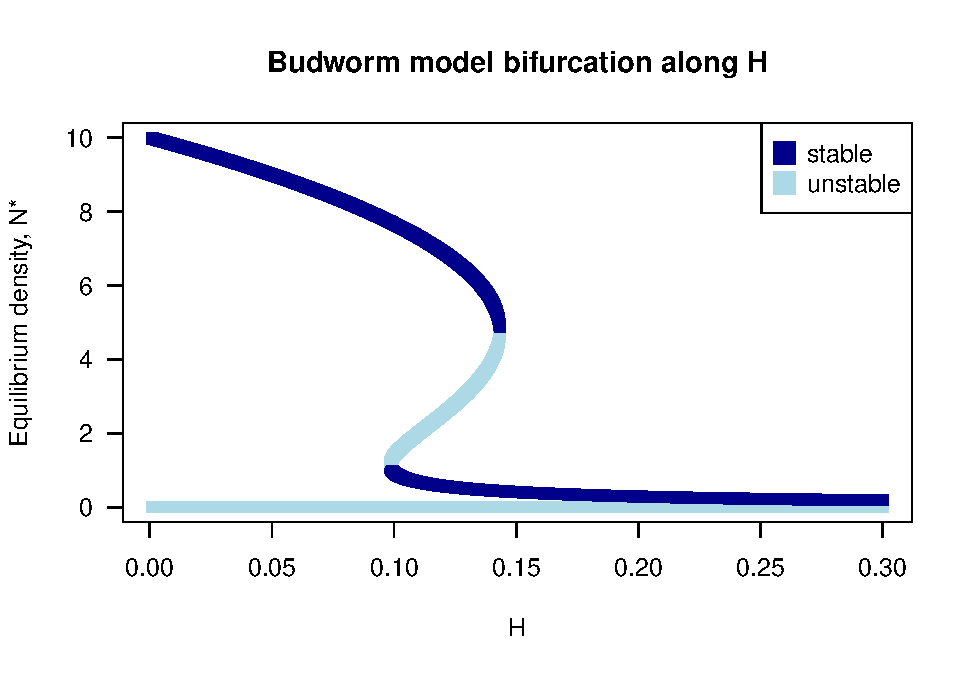
\includegraphics{bookdown-demo_files/figure-latex/unnamed-chunk-20-1.pdf}

\begin{Shaded}
\begin{Highlighting}[]
\DocumentationTok{\#\#\# Visualization II}
\FunctionTok{plot}\NormalTok{(}\FunctionTok{range}\NormalTok{(times), }\FunctionTok{c}\NormalTok{(}\DecValTok{0}\NormalTok{,}\DecValTok{1}\NormalTok{), }\AttributeTok{type =} \StringTok{"n"}\NormalTok{, }\AttributeTok{xlab =} \StringTok{"time"}\NormalTok{, }\AttributeTok{ylab =} \StringTok{"proportion"}\NormalTok{)}
\FunctionTok{lines}\NormalTok{(P00 }\SpecialCharTok{\textasciitilde{}}\NormalTok{ time, }\AttributeTok{data =}\NormalTok{ pop\_size, }\AttributeTok{col =} \StringTok{"tomato"}\NormalTok{)}
\FunctionTok{lines}\NormalTok{(P0A }\SpecialCharTok{\textasciitilde{}}\NormalTok{ time, }\AttributeTok{data =}\NormalTok{ pop\_size, }\AttributeTok{col =} \StringTok{"navy"}\NormalTok{)}
\FunctionTok{lines}\NormalTok{(PA0 }\SpecialCharTok{\textasciitilde{}}\NormalTok{ time, }\AttributeTok{data =}\NormalTok{ pop\_size, }\AttributeTok{col =} \StringTok{"gray"}\NormalTok{)}
\FunctionTok{lines}\NormalTok{(PAA }\SpecialCharTok{\textasciitilde{}}\NormalTok{ time, }\AttributeTok{data =}\NormalTok{ pop\_size, }\AttributeTok{col =} \StringTok{"orange"}\NormalTok{)}
\FunctionTok{legend}\NormalTok{(}\StringTok{"topleft"}\NormalTok{, }\AttributeTok{legend =} \FunctionTok{c}\NormalTok{(}\StringTok{"P00"}\NormalTok{, }\StringTok{"P0A"}\NormalTok{, }\StringTok{"PA0"}\NormalTok{, }\StringTok{"PAA"}\NormalTok{), }\AttributeTok{col =} \FunctionTok{c}\NormalTok{(}\StringTok{"tomato"}\NormalTok{, }\StringTok{"navy"}\NormalTok{, }\StringTok{"gray"}\NormalTok{, }\StringTok{"orange"}\NormalTok{), }\AttributeTok{lty =} \DecValTok{1}\NormalTok{)}
\end{Highlighting}
\end{Shaded}

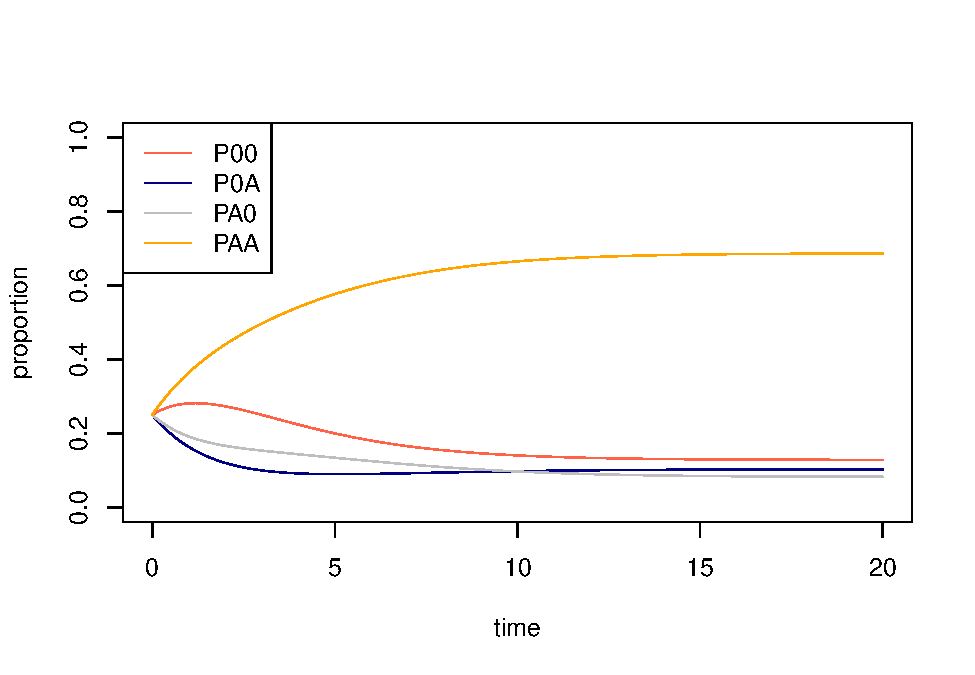
\includegraphics{bookdown-demo_files/figure-latex/unnamed-chunk-20-2.pdf}

\hypertarget{week-7---lotka-volterra-competition-model---population-dynamics}{%
\chapter*{Week 7 - Lotka-Volterra competition model - Population dynamics}\label{week-7---lotka-volterra-competition-model---population-dynamics}}
\addcontentsline{toc}{chapter}{Week 7 - Lotka-Volterra competition model - Population dynamics}

In this lab, we are going to analyze the two-species Lotka-Volterra competition model numerically and visualize the population dynamics under different parameter settings.

\begin{Shaded}
\begin{Highlighting}[]
\FunctionTok{library}\NormalTok{(ggplot2)}
\FunctionTok{library}\NormalTok{(tidyverse)}
\FunctionTok{library}\NormalTok{(deSolve)}

\NormalTok{LV\_model }\OtherTok{\textless{}{-}} \ControlFlowTok{function}\NormalTok{(}\AttributeTok{r1 =} \FloatTok{1.4}\NormalTok{, }\AttributeTok{r2 =} \FloatTok{1.2}\NormalTok{, }\AttributeTok{a11 =} \DecValTok{1}\SpecialCharTok{/}\DecValTok{200}\NormalTok{, }\AttributeTok{a21 =} \DecValTok{1}\SpecialCharTok{/}\DecValTok{400}\NormalTok{, }\AttributeTok{a22 =} \DecValTok{1}\SpecialCharTok{/}\DecValTok{200}\NormalTok{, }\AttributeTok{a12 =} \DecValTok{1}\SpecialCharTok{/}\DecValTok{300}\NormalTok{, }\AttributeTok{N1\_0 =} \DecValTok{10}\NormalTok{, }\AttributeTok{N2\_0 =} \DecValTok{10}\NormalTok{) \{}

  \DocumentationTok{\#\#\# Model specification}
\NormalTok{  LV }\OtherTok{\textless{}{-}} \ControlFlowTok{function}\NormalTok{(times, state, parms) \{}
    \FunctionTok{with}\NormalTok{(}\FunctionTok{as.list}\NormalTok{(}\FunctionTok{c}\NormalTok{(state, parms)), \{}
\NormalTok{      dN1\_dt }\OtherTok{=}\NormalTok{ N1 }\SpecialCharTok{*}\NormalTok{ (r1 }\SpecialCharTok{{-}}\NormalTok{ a11}\SpecialCharTok{*}\NormalTok{N1 }\SpecialCharTok{{-}}\NormalTok{ a12}\SpecialCharTok{*}\NormalTok{N2)}
\NormalTok{      dN2\_dt }\OtherTok{=}\NormalTok{ N2 }\SpecialCharTok{*}\NormalTok{ (r2 }\SpecialCharTok{{-}}\NormalTok{ a22}\SpecialCharTok{*}\NormalTok{N2 }\SpecialCharTok{{-}}\NormalTok{ a21}\SpecialCharTok{*}\NormalTok{N1)}
      \FunctionTok{return}\NormalTok{(}\FunctionTok{list}\NormalTok{(}\FunctionTok{c}\NormalTok{(dN1\_dt, dN2\_dt)))}
\NormalTok{    \})}
\NormalTok{  \}}

  \DocumentationTok{\#\#\# Model parameters}
\NormalTok{  times }\OtherTok{\textless{}{-}} \FunctionTok{seq}\NormalTok{(}\DecValTok{0}\NormalTok{, }\DecValTok{100}\NormalTok{, }\AttributeTok{by =} \FloatTok{0.1}\NormalTok{)}
\NormalTok{  state }\OtherTok{\textless{}{-}} \FunctionTok{c}\NormalTok{(}\AttributeTok{N1 =}\NormalTok{ N1\_0, }\AttributeTok{N2 =}\NormalTok{ N2\_0)}
\NormalTok{  parms }\OtherTok{\textless{}{-}} \FunctionTok{c}\NormalTok{(}\AttributeTok{r1 =}\NormalTok{ r1, }\AttributeTok{r2 =}\NormalTok{ r2, }\AttributeTok{a11 =}\NormalTok{ a11, }\AttributeTok{a21 =}\NormalTok{ a21, }\AttributeTok{a22 =}\NormalTok{ a22, }\AttributeTok{a12 =}\NormalTok{ a12)}

  \DocumentationTok{\#\#\# Model application}
\NormalTok{  pop\_size }\OtherTok{\textless{}{-}} \FunctionTok{ode}\NormalTok{(}\AttributeTok{func =}\NormalTok{ LV, }\AttributeTok{times =}\NormalTok{ times, }\AttributeTok{y =}\NormalTok{ state, }\AttributeTok{parms =}\NormalTok{ parms)}

  \DocumentationTok{\#\#\# Visualize the population dynamics}
\NormalTok{  pop\_size }\SpecialCharTok{\%\textgreater{}\%}
    \FunctionTok{as.data.frame}\NormalTok{() }\SpecialCharTok{\%\textgreater{}\%}
    \FunctionTok{gather}\NormalTok{(}\AttributeTok{key =} \StringTok{"Species"}\NormalTok{, }\AttributeTok{value =} \StringTok{"pop\_size"}\NormalTok{, }\SpecialCharTok{{-}}\NormalTok{time) }\SpecialCharTok{\%\textgreater{}\%}
    \FunctionTok{ggplot}\NormalTok{(}\FunctionTok{aes}\NormalTok{(}\AttributeTok{x =}\NormalTok{ time, }\AttributeTok{y =}\NormalTok{ pop\_size, }\AttributeTok{color =}\NormalTok{ Species)) }\SpecialCharTok{+}
    \FunctionTok{geom\_line}\NormalTok{(}\AttributeTok{size =} \FloatTok{1.5}\NormalTok{)}

\NormalTok{\}}

  \DocumentationTok{\#\#\# Different parameter settings}
  \DocumentationTok{\#\# N1\_0 = 200 and N2\_0 = 5}
  \FunctionTok{LV\_model}\NormalTok{(}\AttributeTok{r1 =} \FloatTok{1.2}\NormalTok{, }\AttributeTok{r2 =} \FloatTok{1.2}\NormalTok{, }\AttributeTok{a11 =} \DecValTok{1}\SpecialCharTok{/}\DecValTok{200}\NormalTok{, }\AttributeTok{a21 =} \DecValTok{1}\SpecialCharTok{/}\DecValTok{100}\NormalTok{, }\AttributeTok{a22 =} \DecValTok{1}\SpecialCharTok{/}\DecValTok{100}\NormalTok{, }\AttributeTok{a12 =} \DecValTok{1}\SpecialCharTok{/}\DecValTok{200}\NormalTok{, }\AttributeTok{N1\_0 =} \DecValTok{200}\NormalTok{, }\AttributeTok{N2\_0 =} \DecValTok{5}\NormalTok{)  }\CommentTok{\# N1 wins}
\end{Highlighting}
\end{Shaded}

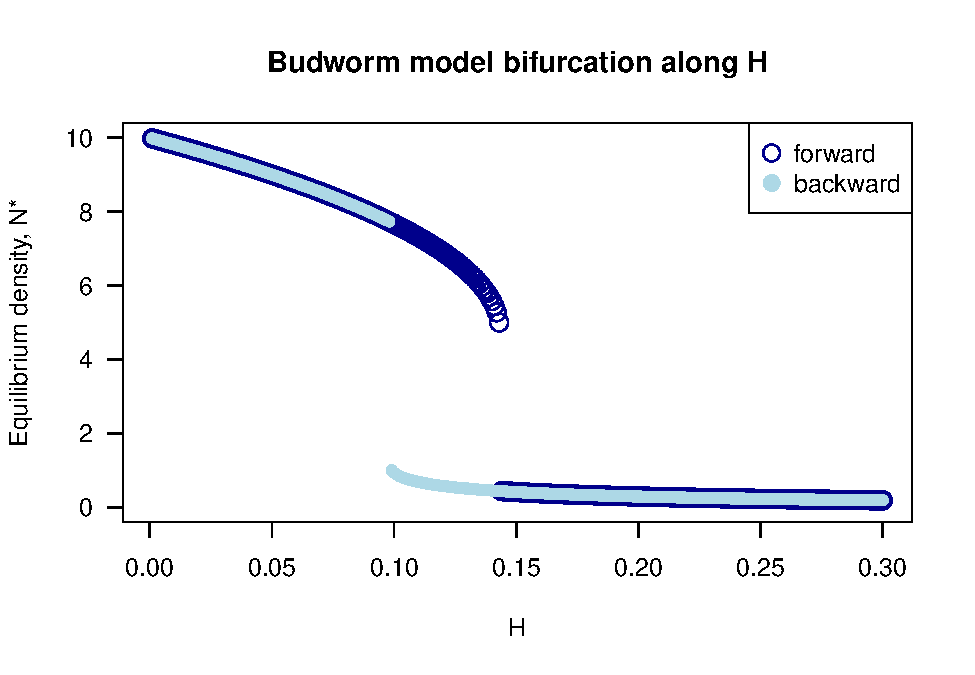
\includegraphics{bookdown-demo_files/figure-latex/unnamed-chunk-21-1.pdf}

\begin{Shaded}
\begin{Highlighting}[]
  \DocumentationTok{\#\# N1\_0 = 5 and N2\_0 = 200}
  \FunctionTok{LV\_model}\NormalTok{(}\AttributeTok{r1 =} \FloatTok{1.2}\NormalTok{, }\AttributeTok{r2 =} \FloatTok{1.2}\NormalTok{, }\AttributeTok{a11 =} \DecValTok{1}\SpecialCharTok{/}\DecValTok{200}\NormalTok{, }\AttributeTok{a21 =} \DecValTok{1}\SpecialCharTok{/}\DecValTok{100}\NormalTok{, }\AttributeTok{a22 =} \DecValTok{1}\SpecialCharTok{/}\DecValTok{100}\NormalTok{, }\AttributeTok{a12 =} \DecValTok{1}\SpecialCharTok{/}\DecValTok{200}\NormalTok{, }\AttributeTok{N1\_0 =} \DecValTok{10}\NormalTok{, }\AttributeTok{N2\_0 =} \DecValTok{200}\NormalTok{)  }\CommentTok{\# N1 wins}
\end{Highlighting}
\end{Shaded}

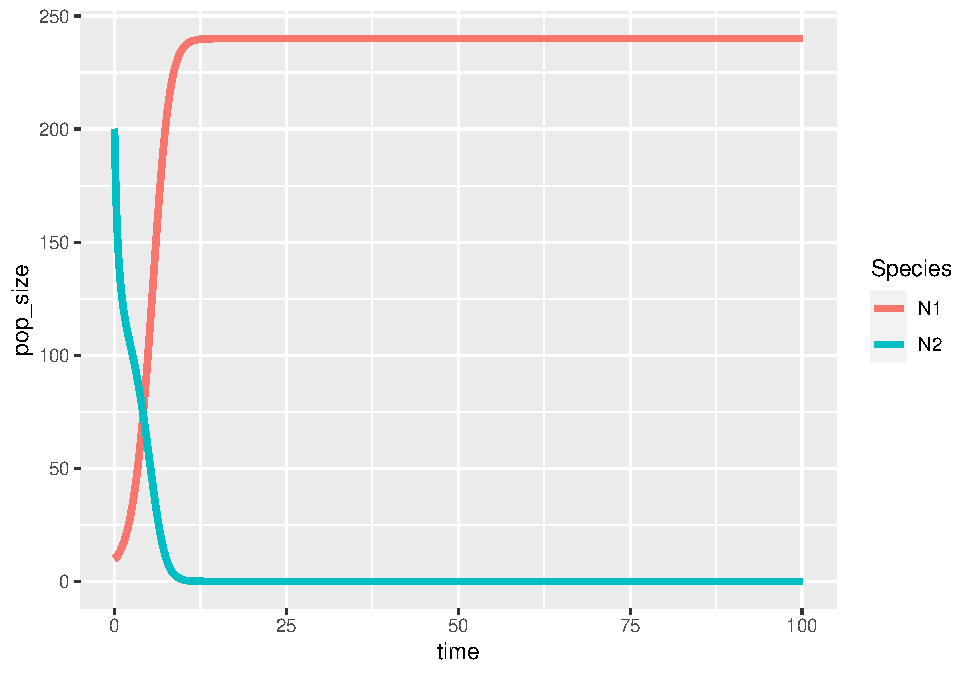
\includegraphics{bookdown-demo_files/figure-latex/unnamed-chunk-21-2.pdf}

\begin{Shaded}
\begin{Highlighting}[]
  \DocumentationTok{\#\# N1\_0 = 200 and N2\_0 = 5}
  \FunctionTok{LV\_model}\NormalTok{(}\AttributeTok{r1 =} \FloatTok{1.2}\NormalTok{, }\AttributeTok{r2 =} \FloatTok{1.2}\NormalTok{, }\AttributeTok{a11 =} \DecValTok{1}\SpecialCharTok{/}\DecValTok{100}\NormalTok{, }\AttributeTok{a21 =} \DecValTok{1}\SpecialCharTok{/}\DecValTok{200}\NormalTok{, }\AttributeTok{a22 =} \DecValTok{1}\SpecialCharTok{/}\DecValTok{200}\NormalTok{, }\AttributeTok{a12 =} \DecValTok{1}\SpecialCharTok{/}\DecValTok{100}\NormalTok{, }\AttributeTok{N1\_0 =} \DecValTok{200}\NormalTok{, }\AttributeTok{N2\_0 =} \DecValTok{5}\NormalTok{)  }\CommentTok{\# N2 wins}
\end{Highlighting}
\end{Shaded}

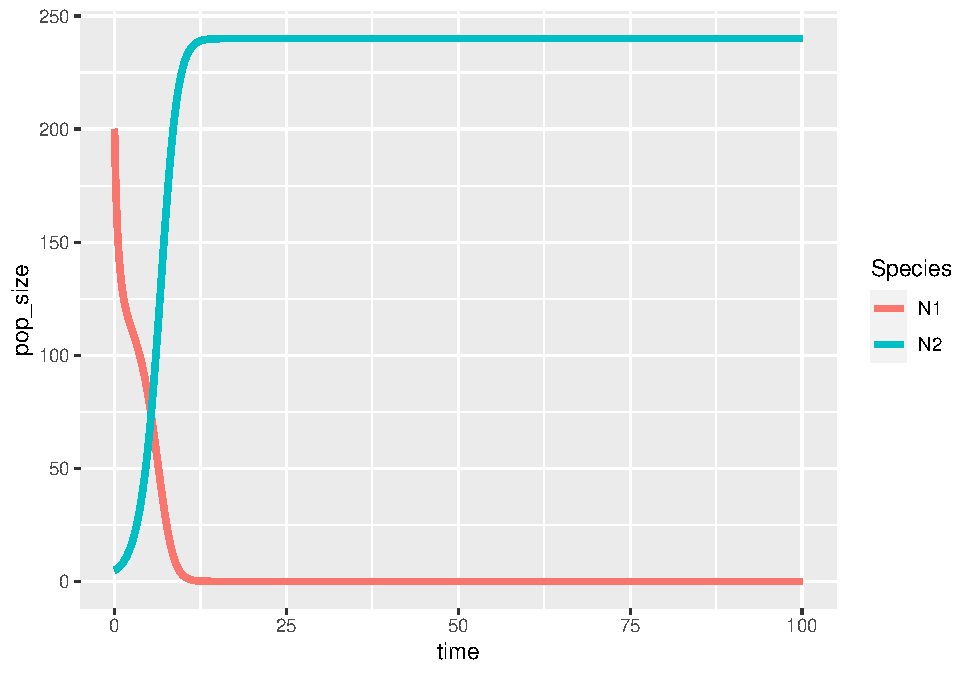
\includegraphics{bookdown-demo_files/figure-latex/unnamed-chunk-21-3.pdf}

\begin{Shaded}
\begin{Highlighting}[]
  \DocumentationTok{\#\# N1\_0 = 5 and N2\_0 = 200}
  \FunctionTok{LV\_model}\NormalTok{(}\AttributeTok{r1 =} \FloatTok{1.2}\NormalTok{, }\AttributeTok{r2 =} \FloatTok{1.2}\NormalTok{, }\AttributeTok{a11 =} \DecValTok{1}\SpecialCharTok{/}\DecValTok{100}\NormalTok{, }\AttributeTok{a21 =} \DecValTok{1}\SpecialCharTok{/}\DecValTok{200}\NormalTok{, }\AttributeTok{a22 =} \DecValTok{1}\SpecialCharTok{/}\DecValTok{200}\NormalTok{, }\AttributeTok{a12 =} \DecValTok{1}\SpecialCharTok{/}\DecValTok{100}\NormalTok{, }\AttributeTok{N1\_0 =} \DecValTok{5}\NormalTok{, }\AttributeTok{N2\_0 =} \DecValTok{200}\NormalTok{)  }\CommentTok{\# N2 wins}
\end{Highlighting}
\end{Shaded}

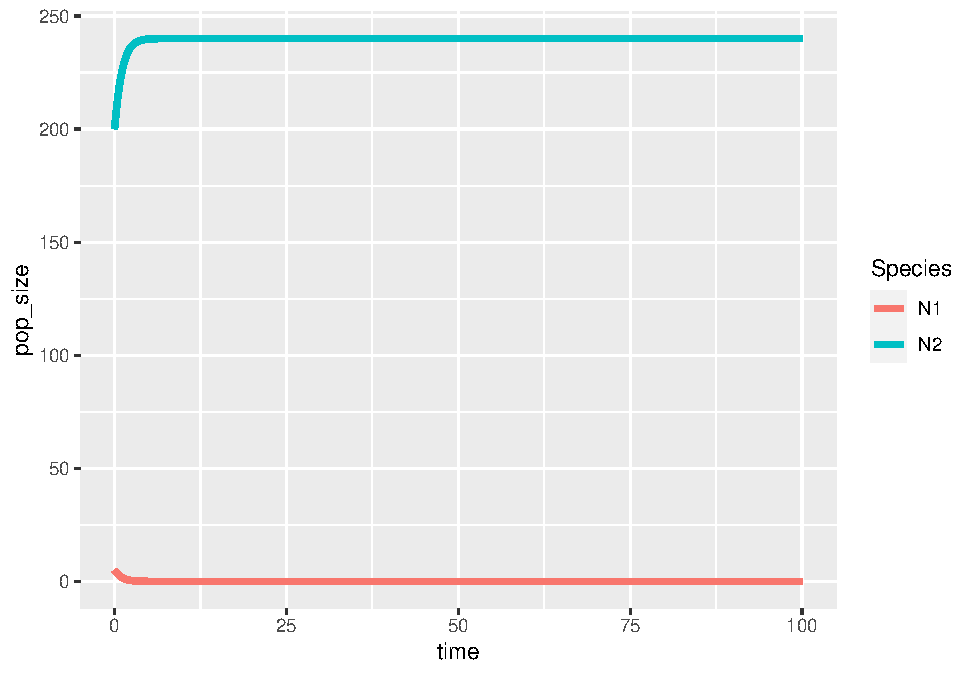
\includegraphics{bookdown-demo_files/figure-latex/unnamed-chunk-21-4.pdf}

\begin{Shaded}
\begin{Highlighting}[]
  \DocumentationTok{\#\# N1\_0 = 200 and N2\_0 = 5}
  \FunctionTok{LV\_model}\NormalTok{(}\AttributeTok{r1 =} \FloatTok{1.2}\NormalTok{, }\AttributeTok{r2 =} \FloatTok{1.2}\NormalTok{, }\AttributeTok{a11 =} \DecValTok{1}\SpecialCharTok{/}\DecValTok{100}\NormalTok{, }\AttributeTok{a21 =} \DecValTok{1}\SpecialCharTok{/}\DecValTok{200}\NormalTok{, }\AttributeTok{a22 =} \DecValTok{1}\SpecialCharTok{/}\DecValTok{100}\NormalTok{, }\AttributeTok{a12 =} \DecValTok{1}\SpecialCharTok{/}\DecValTok{300}\NormalTok{, }\AttributeTok{N1\_0 =} \DecValTok{200}\NormalTok{, }\AttributeTok{N2\_0 =} \DecValTok{5}\NormalTok{)  }\CommentTok{\# stable coexistence}
\end{Highlighting}
\end{Shaded}

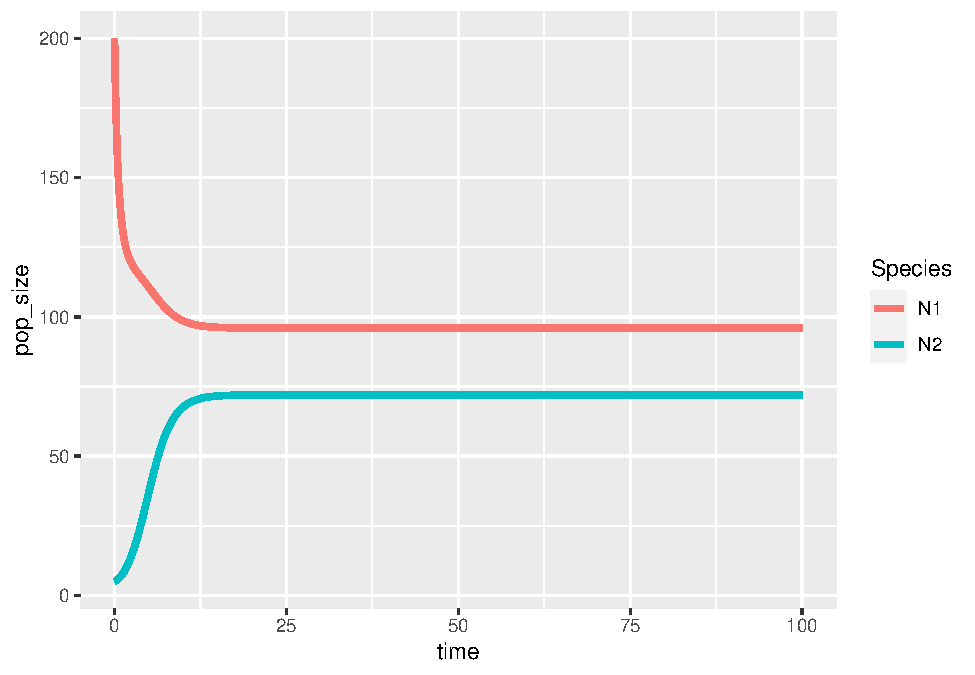
\includegraphics{bookdown-demo_files/figure-latex/unnamed-chunk-21-5.pdf}

\begin{Shaded}
\begin{Highlighting}[]
  \DocumentationTok{\#\# N1\_0 = 5 and N2\_0 = 200}
  \FunctionTok{LV\_model}\NormalTok{(}\AttributeTok{r1 =} \FloatTok{1.2}\NormalTok{, }\AttributeTok{r2 =} \FloatTok{1.2}\NormalTok{, }\AttributeTok{a11 =} \DecValTok{1}\SpecialCharTok{/}\DecValTok{100}\NormalTok{, }\AttributeTok{a21 =} \DecValTok{1}\SpecialCharTok{/}\DecValTok{200}\NormalTok{, }\AttributeTok{a22 =} \DecValTok{1}\SpecialCharTok{/}\DecValTok{100}\NormalTok{, }\AttributeTok{a12 =} \DecValTok{1}\SpecialCharTok{/}\DecValTok{300}\NormalTok{, }\AttributeTok{N1\_0 =} \DecValTok{5}\NormalTok{, }\AttributeTok{N2\_0 =} \DecValTok{200}\NormalTok{)  }\CommentTok{\# stable coexistence}
\end{Highlighting}
\end{Shaded}

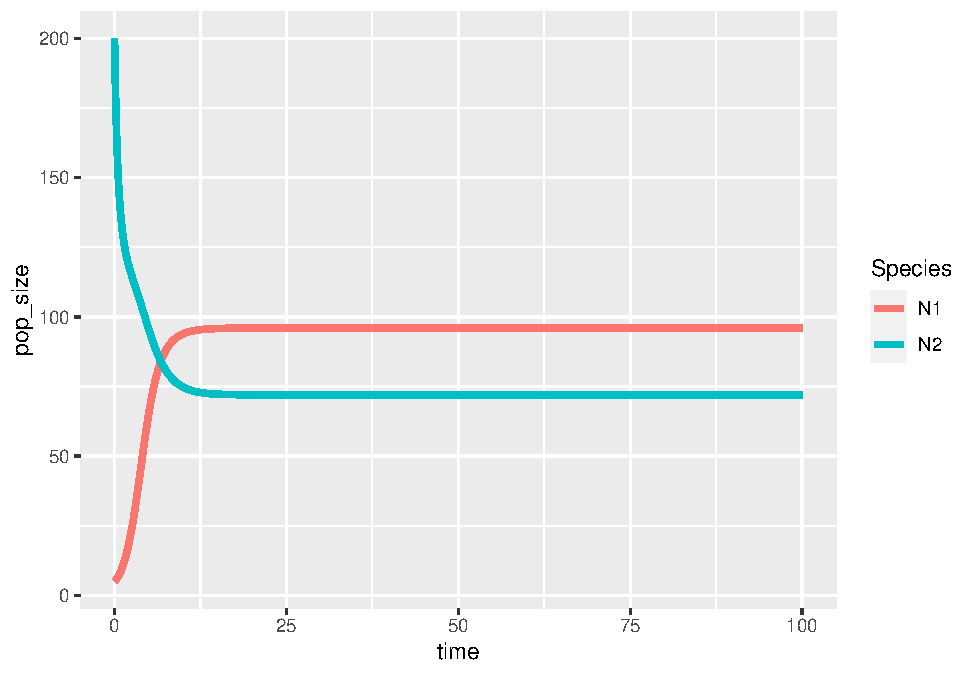
\includegraphics{bookdown-demo_files/figure-latex/unnamed-chunk-21-6.pdf}

\begin{Shaded}
\begin{Highlighting}[]
  \DocumentationTok{\#\# N1\_0 = 200 and N2\_0 = 150}
  \FunctionTok{LV\_model}\NormalTok{(}\AttributeTok{r1 =} \FloatTok{1.2}\NormalTok{, }\AttributeTok{r2 =} \FloatTok{1.2}\NormalTok{, }\AttributeTok{a11 =} \DecValTok{1}\SpecialCharTok{/}\DecValTok{200}\NormalTok{, }\AttributeTok{a21 =} \DecValTok{1}\SpecialCharTok{/}\DecValTok{100}\NormalTok{, }\AttributeTok{a22 =} \DecValTok{1}\SpecialCharTok{/}\DecValTok{200}\NormalTok{, }\AttributeTok{a12 =} \DecValTok{1}\SpecialCharTok{/}\DecValTok{100}\NormalTok{, }\AttributeTok{N1\_0 =} \DecValTok{200}\NormalTok{, }\AttributeTok{N2\_0 =} \DecValTok{150}\NormalTok{)  }\CommentTok{\# priority effect (N1 wins)}
\end{Highlighting}
\end{Shaded}

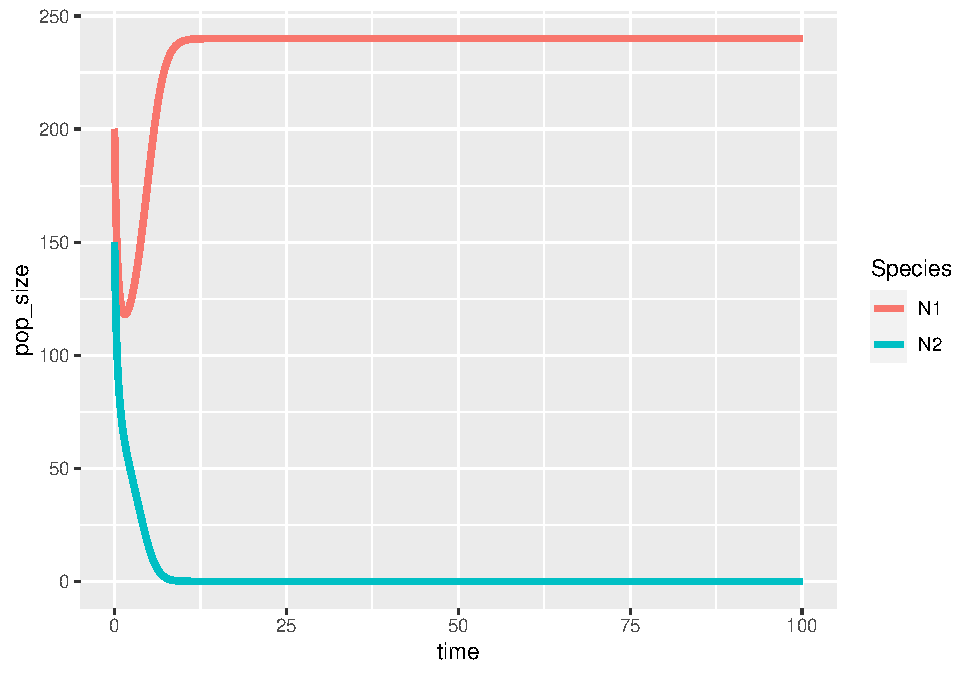
\includegraphics{bookdown-demo_files/figure-latex/unnamed-chunk-21-7.pdf}

\begin{Shaded}
\begin{Highlighting}[]
  \DocumentationTok{\#\# N1\_0 = 150 and N2\_0 = 200}
  \FunctionTok{LV\_model}\NormalTok{(}\AttributeTok{r1 =} \FloatTok{1.2}\NormalTok{, }\AttributeTok{r2 =} \FloatTok{1.2}\NormalTok{, }\AttributeTok{a11 =} \DecValTok{1}\SpecialCharTok{/}\DecValTok{200}\NormalTok{, }\AttributeTok{a21 =} \DecValTok{1}\SpecialCharTok{/}\DecValTok{100}\NormalTok{, }\AttributeTok{a22 =} \DecValTok{1}\SpecialCharTok{/}\DecValTok{200}\NormalTok{, }\AttributeTok{a12 =} \DecValTok{1}\SpecialCharTok{/}\DecValTok{100}\NormalTok{, }\AttributeTok{N1\_0 =} \DecValTok{150}\NormalTok{, }\AttributeTok{N2\_0 =} \DecValTok{200}\NormalTok{)  }\CommentTok{\# priority effect (N2 wins)}
\end{Highlighting}
\end{Shaded}

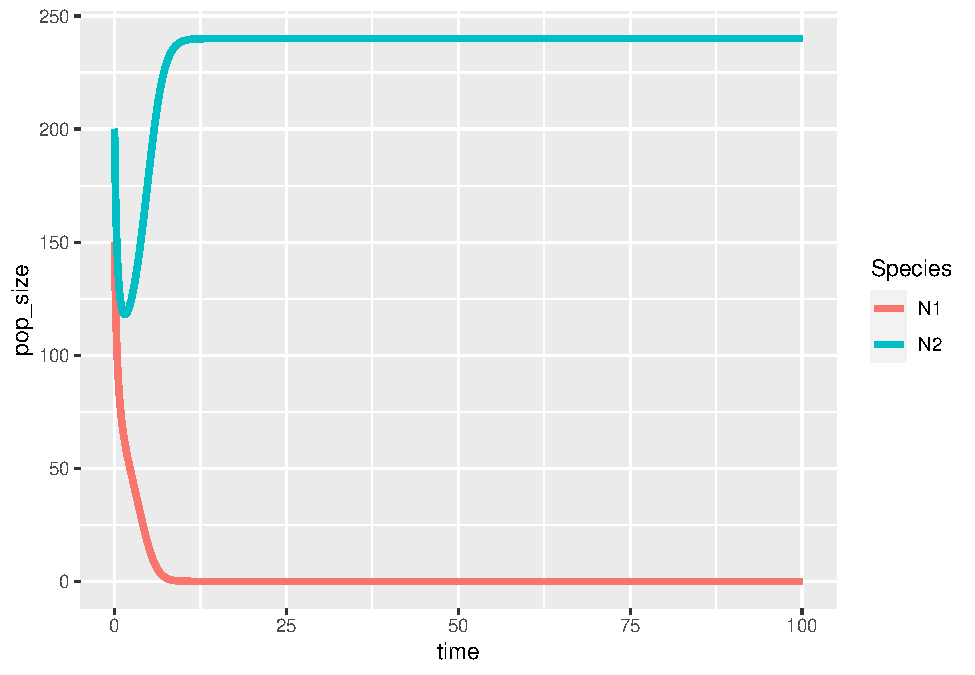
\includegraphics{bookdown-demo_files/figure-latex/unnamed-chunk-21-8.pdf}

\begin{Shaded}
\begin{Highlighting}[]
\DocumentationTok{\#\#\#\# phase diagram}
\NormalTok{phase\_plane }\OtherTok{\textless{}{-}} \ControlFlowTok{function}\NormalTok{(r1, r2, a11, a21, a22, a12, title, t)\{}
    \DocumentationTok{\#\#\# Vectors}
\NormalTok{  LV }\OtherTok{\textless{}{-}} \ControlFlowTok{function}\NormalTok{(times, state, parms) \{}
    \FunctionTok{with}\NormalTok{(}\FunctionTok{as.list}\NormalTok{(}\FunctionTok{c}\NormalTok{(state, parms)), \{}
\NormalTok{      dN1\_dt }\OtherTok{=}\NormalTok{ N1 }\SpecialCharTok{*}\NormalTok{ (r1 }\SpecialCharTok{{-}}\NormalTok{ a11}\SpecialCharTok{*}\NormalTok{N1 }\SpecialCharTok{{-}}\NormalTok{ a12}\SpecialCharTok{*}\NormalTok{N2)}
\NormalTok{      dN2\_dt }\OtherTok{=}\NormalTok{ N2 }\SpecialCharTok{*}\NormalTok{ (r2 }\SpecialCharTok{{-}}\NormalTok{ a22}\SpecialCharTok{*}\NormalTok{N2 }\SpecialCharTok{{-}}\NormalTok{ a21}\SpecialCharTok{*}\NormalTok{N1)}
      \FunctionTok{return}\NormalTok{(}\FunctionTok{list}\NormalTok{(}\FunctionTok{c}\NormalTok{(dN1\_dt, dN2\_dt)))}
\NormalTok{    \})}
\NormalTok{  \}}

\NormalTok{  times }\OtherTok{\textless{}{-}} \FunctionTok{c}\NormalTok{(}\DecValTok{0}\NormalTok{, t)}
\NormalTok{  parms }\OtherTok{\textless{}{-}} \FunctionTok{c}\NormalTok{(}\AttributeTok{r1 =}\NormalTok{ r1, }\AttributeTok{r2 =}\NormalTok{ r2, }\AttributeTok{a11 =}\NormalTok{ a11, }\AttributeTok{a21 =}\NormalTok{ a21, }\AttributeTok{a22 =}\NormalTok{ a22, }\AttributeTok{a12 =}\NormalTok{ a12)}

\NormalTok{  x\_inter}\OtherTok{\textless{}{-}} \FunctionTok{max}\NormalTok{(}\FunctionTok{c}\NormalTok{(r1}\SpecialCharTok{/}\NormalTok{a11, r2}\SpecialCharTok{/}\NormalTok{a21))}
\NormalTok{  y\_inter }\OtherTok{\textless{}{-}} \FunctionTok{max}\NormalTok{(}\FunctionTok{c}\NormalTok{(r2}\SpecialCharTok{/}\NormalTok{a22, r1}\SpecialCharTok{/}\NormalTok{a12))}

  \CommentTok{\# create position of arrows}
\NormalTok{  vector\_grid }\OtherTok{\textless{}{-}} \FunctionTok{expand.grid}\NormalTok{(}\FunctionTok{seq}\NormalTok{(}\DecValTok{5}\NormalTok{, x\_inter, }\AttributeTok{length.out =} \DecValTok{10}\NormalTok{),}
                             \FunctionTok{seq}\NormalTok{(}\DecValTok{5}\NormalTok{, y\_inter, }\AttributeTok{length.out =} \DecValTok{10}\NormalTok{))}

\NormalTok{  vector\_data }\OtherTok{\textless{}{-}}\NormalTok{ vector\_grid }\SpecialCharTok{\%\textgreater{}\%}
    \FunctionTok{pmap}\NormalTok{(., }\ControlFlowTok{function}\NormalTok{(Var1, Var2)\{}
\NormalTok{      state }\OtherTok{\textless{}{-}} \FunctionTok{c}\NormalTok{(}\AttributeTok{N1 =}\NormalTok{ Var1, }\AttributeTok{N2 =}\NormalTok{ Var2)}
\NormalTok{      pop\_size }\OtherTok{\textless{}{-}} \FunctionTok{ode}\NormalTok{(}\AttributeTok{func =}\NormalTok{ LV, }\AttributeTok{times =}\NormalTok{ times, }\AttributeTok{y =}\NormalTok{ state, }\AttributeTok{parms =}\NormalTok{ parms)}
\NormalTok{      pop\_size[}\DecValTok{2}\NormalTok{, }\DecValTok{2}\SpecialCharTok{:}\DecValTok{3}\NormalTok{]}
\NormalTok{    \}) }\SpecialCharTok{\%\textgreater{}\%}
    \FunctionTok{bind\_rows}\NormalTok{() }\SpecialCharTok{\%\textgreater{}\%}
    \FunctionTok{rename}\NormalTok{(}\AttributeTok{xend =}\NormalTok{ N1, }\AttributeTok{yend =}\NormalTok{ N2) }\SpecialCharTok{\%\textgreater{}\%}
    \FunctionTok{bind\_cols}\NormalTok{(vector\_grid) }\SpecialCharTok{\%\textgreater{}\%}
    \FunctionTok{rename}\NormalTok{(}\AttributeTok{x =}\NormalTok{ Var1, }\AttributeTok{y =}\NormalTok{ Var2)}

    \DocumentationTok{\#\#\# Phase plane}
    \FunctionTok{ggplot}\NormalTok{() }\SpecialCharTok{+}
      \FunctionTok{geom\_abline}\NormalTok{(}\AttributeTok{slope =} \SpecialCharTok{{-}}\NormalTok{a11}\SpecialCharTok{/}\NormalTok{a12, }\AttributeTok{intercept =}\NormalTok{ r1}\SpecialCharTok{/}\NormalTok{a12, }\AttributeTok{color =} \StringTok{"\#E41A1C"}\NormalTok{, }\AttributeTok{size =} \FloatTok{1.5}\NormalTok{) }\SpecialCharTok{+}
      \FunctionTok{geom\_abline}\NormalTok{(}\AttributeTok{slope =} \SpecialCharTok{{-}}\NormalTok{a21}\SpecialCharTok{/}\NormalTok{a22, }\AttributeTok{intercept =}\NormalTok{ r2}\SpecialCharTok{/}\NormalTok{a22, }\AttributeTok{color =} \StringTok{"\#377EB8"}\NormalTok{, }\AttributeTok{size =} \FloatTok{1.5}\NormalTok{) }\SpecialCharTok{+}
      \FunctionTok{geom\_segment}\NormalTok{(}\AttributeTok{data =}\NormalTok{ vector\_data,}
                   \FunctionTok{aes}\NormalTok{(}\AttributeTok{x =}\NormalTok{ x, }\AttributeTok{y =}\NormalTok{ y, }\AttributeTok{xend =}\NormalTok{ xend, }\AttributeTok{yend =}\NormalTok{ yend),}
                   \AttributeTok{arrow =} \FunctionTok{arrow}\NormalTok{(}\AttributeTok{length =} \FunctionTok{unit}\NormalTok{(}\FloatTok{0.1}\NormalTok{, }\StringTok{"cm"}\NormalTok{))) }\SpecialCharTok{+}    
      \FunctionTok{scale\_x\_continuous}\NormalTok{(}\AttributeTok{name =} \StringTok{"N1"}\NormalTok{, }\AttributeTok{limits =} \FunctionTok{c}\NormalTok{(}\DecValTok{0}\NormalTok{, x\_inter), }\AttributeTok{expand =} \FunctionTok{c}\NormalTok{(}\DecValTok{0}\NormalTok{, }\DecValTok{0}\NormalTok{)) }\SpecialCharTok{+}
      \FunctionTok{scale\_y\_continuous}\NormalTok{(}\AttributeTok{name =} \StringTok{"N2"}\NormalTok{, }\AttributeTok{limits =} \FunctionTok{c}\NormalTok{(}\DecValTok{0}\NormalTok{, y\_inter), }\AttributeTok{expand =} \FunctionTok{c}\NormalTok{(}\DecValTok{0}\NormalTok{, }\DecValTok{0}\NormalTok{)) }\SpecialCharTok{+}
      \FunctionTok{theme\_bw}\NormalTok{(}\AttributeTok{base\_size =} \DecValTok{13}\NormalTok{) }\SpecialCharTok{+}
      \FunctionTok{theme}\NormalTok{(}\AttributeTok{panel.grid =} \FunctionTok{element\_blank}\NormalTok{(),}
            \AttributeTok{plot.title =} \FunctionTok{element\_text}\NormalTok{(}\AttributeTok{hjust =} \FloatTok{0.5}\NormalTok{)) }\SpecialCharTok{+}
      \FunctionTok{labs}\NormalTok{(}\AttributeTok{title =}\NormalTok{ title)}
\NormalTok{  \}}

  \FunctionTok{phase\_plane}\NormalTok{(}\AttributeTok{r1 =} \FloatTok{1.2}\NormalTok{, }\AttributeTok{r2 =} \FloatTok{1.2}\NormalTok{, }\AttributeTok{a11 =} \DecValTok{1}\SpecialCharTok{/}\DecValTok{100}\NormalTok{, }\AttributeTok{a21 =} \DecValTok{1}\SpecialCharTok{/}\DecValTok{200}\NormalTok{, }\AttributeTok{a22 =} \DecValTok{1}\SpecialCharTok{/}\DecValTok{100}\NormalTok{, }\AttributeTok{a12 =} \DecValTok{1}\SpecialCharTok{/}\DecValTok{300}\NormalTok{, }\AttributeTok{t =} \FloatTok{0.3}\NormalTok{, }\AttributeTok{title =} \StringTok{"Stable coexistence"}\NormalTok{)}
\end{Highlighting}
\end{Shaded}

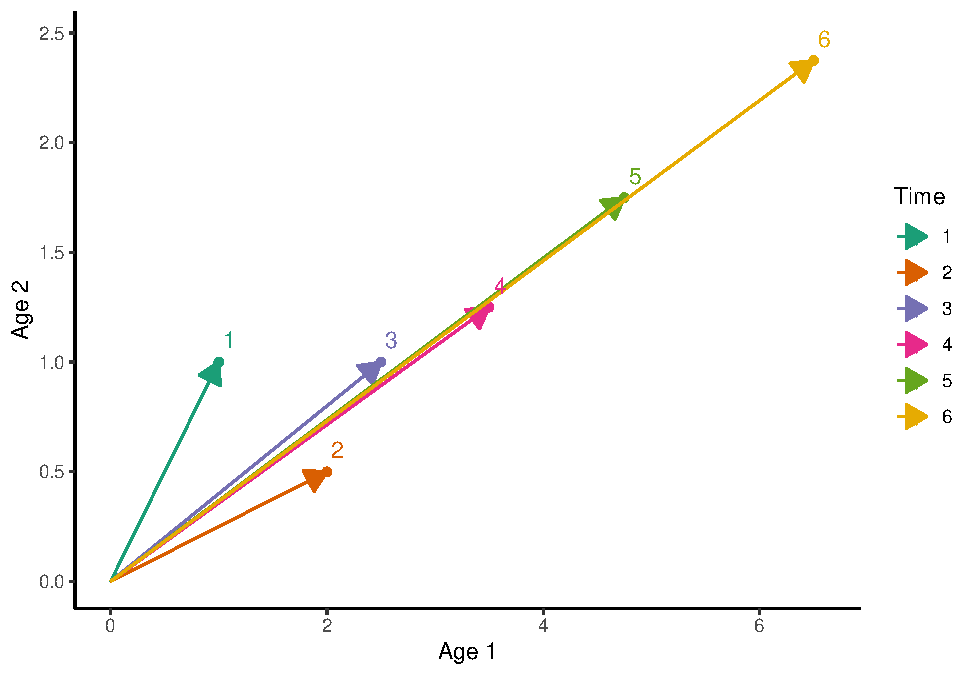
\includegraphics{bookdown-demo_files/figure-latex/unnamed-chunk-22-1.pdf}

\begin{Shaded}
\begin{Highlighting}[]
  \FunctionTok{phase\_plane}\NormalTok{(}\AttributeTok{r1 =} \FloatTok{1.2}\NormalTok{, }\AttributeTok{r2 =} \FloatTok{1.2}\NormalTok{, }\AttributeTok{a11 =} \DecValTok{1}\SpecialCharTok{/}\DecValTok{200}\NormalTok{, }\AttributeTok{a21 =} \DecValTok{1}\SpecialCharTok{/}\DecValTok{100}\NormalTok{, }\AttributeTok{a22 =} \DecValTok{1}\SpecialCharTok{/}\DecValTok{200}\NormalTok{, }\AttributeTok{a12 =} \DecValTok{1}\SpecialCharTok{/}\DecValTok{100}\NormalTok{, }\AttributeTok{t =} \FloatTok{0.3}\NormalTok{, }\AttributeTok{title =} \StringTok{"Unstable coexistence (saddle)"}\NormalTok{)}
\end{Highlighting}
\end{Shaded}

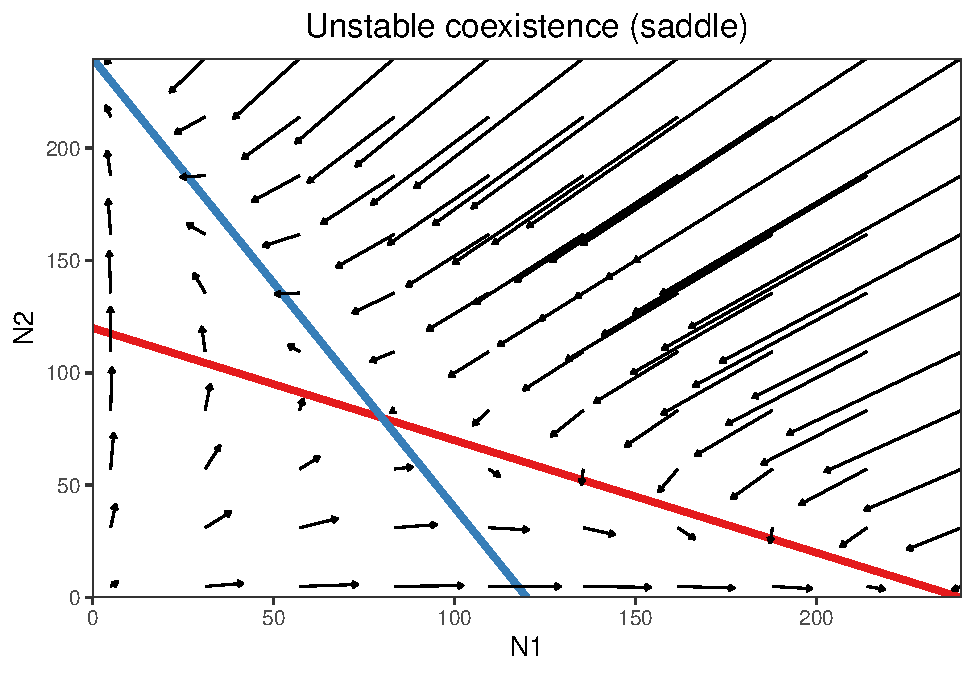
\includegraphics{bookdown-demo_files/figure-latex/unnamed-chunk-22-2.pdf}

\hypertarget{week-8---midterm}{%
\chapter*{Week 8 - Midterm}\label{week-8---midterm}}
\addcontentsline{toc}{chapter}{Week 8 - Midterm}

  \bibliography{book.bib,packages.bib}

\end{document}
